\documentclass[times, twoside]{zHenriquesLab-StyleBioRxiv}

\usepackage{blindtext}
\usepackage{subcaption} % nel preambolo

% Please give the surname of the lead author for the running footer
\leadauthor{Prof. Daniele Fontanelli} 

\begin{document}

\title{Swarm Intelligence and Target Search}
\shorttitle{Swarm Intelligence and Target Search}

% Use letters for affiliations, numbers to show equal authorship (if applicable) and to indicate the corresponding author
\author[1]{Alessandro Rossi}
\author[1]{Lorenzo Franco}

\affil[1]{Intelligent Distributed Systems, master's degree in mechatronics engineering, University of Trento}

\maketitle

%TC:break Abstract
%the command above serves to have a word count for the abstract
\begin{abstract}
Abstract -- A "treasure hunt" can be a fun and engaging opportunity to test the capabilities of a swarm of robots in a simulated environment.
The multiagent system proposed in this project is designed to search for a target in a 2D environment using a combination of swarm
intelligence \cite{consensusUSATO,consensus_A_SCHEME}, Voronoi cells \cite{fontanelli,raycast, Loyd_usato}, Lévy flight \cite{levyUSED,levyDISTRIB} and sensor fusion techniques. The main objective of the project is to
evaluate the performance of the proposed multiagent system in terms of search efficiency, convergence time, and robustness to
noise and uncertainties in the environment. The simulation will be implemented in Python, and the results will be analyzed to draw
conclusions about the effectiveness of the proposed approach in solving the treasure hunt problem.
\end {abstract}
%TC:break main
%the command above serves to have a word count for the abstract

% \begin{keywords}
% Swarm Intelligence, Voronoi Cells, Lévy Flight, Sensor Fusion
% \end{keywords}

% \begin{corrauthor}
% %\texttt{r.henriques{@}ucl.ac.uk}
% r.henriques\at ucl.ac.uk
% \end{corrauthor}

\section*{Introduction}
This project presents a control framework for a swarm of mobile robots
that finds, estimates and encircles a target. The system combines a
LiDAR, for obstacle detection, an Extended Kalman Filter (EKF) for state
estimation and linear consensus for coordination. The treasure is supposed to be a point object emitting a weak radio signal, the detection is performed by a
simple thresholding to detect if the signal is recieved or not. The robots are able
to coordinate their movements unsign a control scheme dictated by a Finite State Machine, allowing convergence to the estimated position of the target
while avoiding obstacles. An iteration of the consensus algorithm enhances the precision of the target estimate. The performance of the proposed control
framework is evaluated through simulations in a 2D environment,
where the robots are tasked with finding and aligning around a target
while navigating through a cluttered environment. The results show
that the proposed approach is effective in enabling the swarm of robots
to find and align around the target, even in the presence of noise and
uncertainties in the environment.

\section*{The Task}

The objective of this project is the localization of a target, modeled as a point object, within a two-dimensional environment. The problem is framed in the context of distributed cooperative control for a team of autonomous mobile robots.
The proposed framework integrates four main components: a Voronoi--Lloyd partitioning scheme, an Extended Kalman Filter (EKF), a Finite State Machine for the control and a linear consensus algorithm. The EKF is employed for sensor fusion, combining dead-reckoning data with camera-based position measurements. The robotic swarm is required to explore the environment, avoid obstacles, detect the target, and finally, converge and align around it.

\subsection*{Structure and Workflow}

The simulation takes place in a 2D environment populated with obstacles, representing a cluttered indoor scenario. A finite state machine (FSM) governs the behavior of each robot. The operational states are defined as follows:

\begin{itemize}[noitemsep]
    \item Searching: Robots explore the environment using a Lévy flight strategy, while actively avoiding collisions with obstacles and other agents.
    
    \item Inspecting: Upon detecting an obstacle, a robot performs local mapping. It also verifies whether the detected object is the target by approaching it and checking for the presence of a radio signal.
    
    \item Target Found: Once the target is identified, all agents converge toward its estimated position. The estimate is progressively refined through iterations of the consensus algorithm.
\end{itemize}

State estimation is achieved via sensor fusion using the EKF, which combines velocity-based dead-reckoning with measurements from a fixed camera located in the top-right corner of the environment (purple square in Figure~\ref{fig:environment}). 

Voronoi cells are computed and used within the control logic of the FSM to improve spatial coordination among robots. 

Additionally, agents communicate with one another by broadcasting messages that include: the position estimate provided by the EKF, locally mapped points contributing to a global map of the environment, and, once detected, the estimated position of the target.

\begin{figure}[H]
\centering
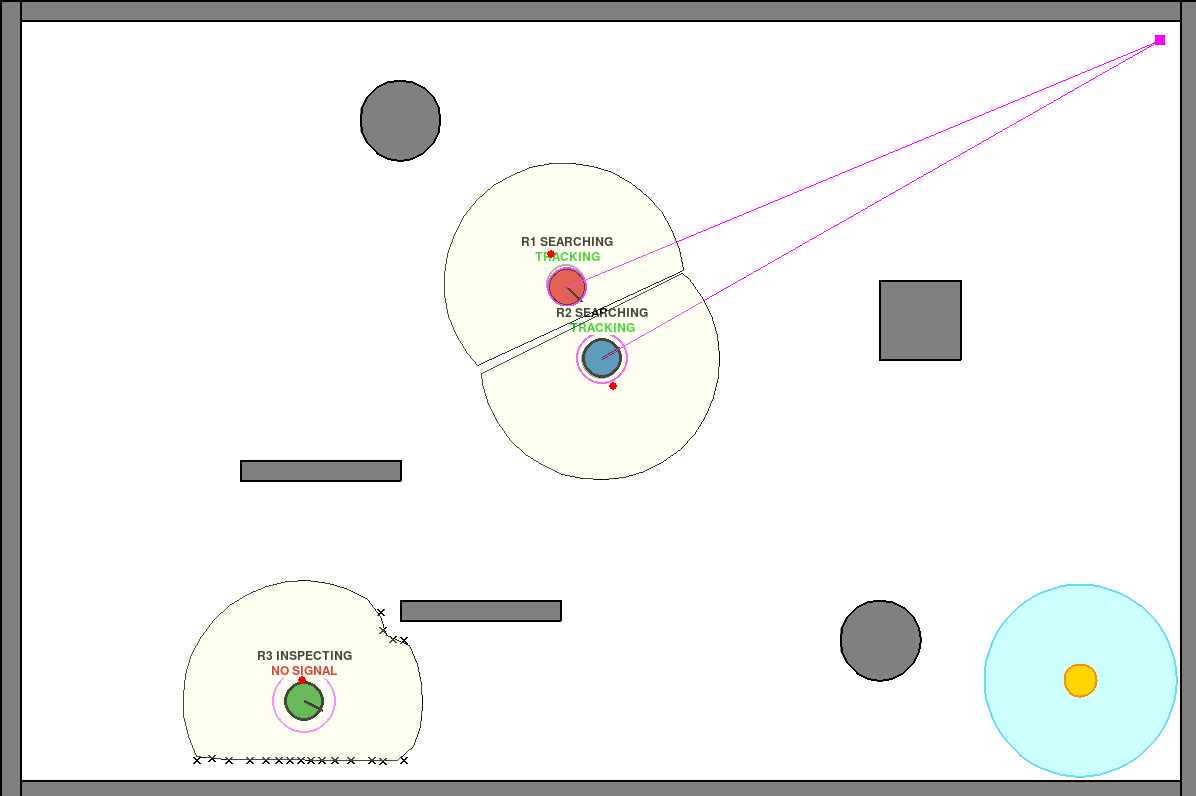
\includegraphics[width=.8\linewidth]{Figures/environment.png}
\caption{Simulation environment}
\label{fig:environment}
\end{figure}

The target object (represented by the yellow area in Fig.~\ref{fig:environment}) cannot be sensed globally by the swarm. Instead, an agent detects the target only upon entering its localized emission range (blue circular region in Fig.~\ref{fig:environment}). Once inside this area, the robot estimates the target's position using a LiDAR sensor. For simplicity, the treasure is abstracted as a dimensionless point. This design choice was implemented to faithfully replicate the physical limitations inherent to real-world sensory systems, such as the bounded propagation radius of localized radio-frequency beacons.

The number of agents, the obstacles shape and position, the room size and the target position are user defined.

Each aspect described above will be discussed in the following sections of the report.






\section*{Model and methods}

\subsection{Motion Model}

The agents operate in a planar environment and are therefore modeled in two dimensions. The state of each robot is defined as:

\begin{equation}
    \mathbf{s} = 
    \begin{bmatrix}
        x \\
        y \\
        \theta
    \end{bmatrix}
\end{equation}

where $(x, y)$ represents the position of the robot in the plane, and $\theta$ denotes its orientation with respect to a global reference frame.

To describe the motion of the robots, the unicycle kinematic model is adopted. The corresponding nonlinear dynamics are given by:

\begin{equation}
\mathbf{\dot{s}} =
\left[
\begin{aligned}
    \dot{x} &= v \cos\theta \\
    \dot{y} &= v \sin\theta \\
    \dot{\theta} &= \omega
\end{aligned}
\right]
\label{eq:unicycle}
\end{equation}

where $v$ is the linear velocity and $\omega$ is the angular velocity, which together form the control input vector:

\begin{equation}
    \mathbf{u} =
    \begin{bmatrix}
        v \\
        \omega
    \end{bmatrix}
    \label{eq:control}
\end{equation}

The unicycle model represents a simplified yet realistic approximation of the robot dynamics. In particular, it captures the nonholonomic constraint that prevents lateral motion, meaning the robot cannot move directly sideways. Despite its simplicity, this model is widely used in mobile robotics, as it effectively captures the behavior of differential-drive robots and similar platforms, while remaining computationally efficient for control and estimation purposes. For these reasons, it was selected for this work.


To improve the realism of the model, disturbances are introduced in the control inputs (Eq.\ref{eq:control}). In practice, uncertainties in differential-drive robots mainly arise from actuation errors, such as wheel slippage, surface irregularities, and imperfect motor response.

The discrete-time version of Eq.~\ref{eq:unicycle} are therefore modeled as:
\begin{equation}
    \mathbf{s}_{k+1} = f(\mathbf{s}_k, \mathbf{u}_k, \boldsymbol{\nu}_k)
\label{eq:f_suv}
\end{equation}

where the process noise $\boldsymbol{\nu}_k$ is assumed Gaussian:
\begin{equation}
    \boldsymbol{\nu}_k \sim \mathcal{N}(\mathbf{0}, \mathbf{Q})
    \label{eq:process_noise}
\end{equation}

The covariance matrix is chosen diagonal:
\begin{equation}
    \mathbf{Q} =
    \begin{bmatrix}
        \sigma_v^2 & 0 \\
        0 & \sigma_\omega^2
    \end{bmatrix}
\end{equation}

Thus, the relation (Eq.~\ref{eq:f_suv}) can be written as:
\begin{equation}
\label{eq:discr_unicycle}
\begin{bmatrix}
    x_{k+1} \\
    y_{k+1} \\
    \theta_{k+1}
\end{bmatrix}
=
\begin{bmatrix}
    x_k \\
    y_k \\
    \theta_k
\end{bmatrix}
+
\begin{bmatrix}
    \cos\theta_k & 0 \\
    \sin\theta_k & 0 \\
    0 & 1
\end{bmatrix}
\Delta t
\left(
\begin{bmatrix}
    v_k \\
    \omega_k
\end{bmatrix}
+
\boldsymbol{\nu}_k
\right)
\end{equation}

\subsection{Measurement and Sensing Model}

The robots are assumed to be equipped with the following sensing systems:

\begin{itemize}[noitemsep]
    
    \item Camera-based position measurements: used in the update step of the EKF. A fixed camera observes the robots (e.g., through ArUco markers) and provides an estimate of their full pose in the global reference frame.
    \\
    
    The measurement model is therefore defined as:
\begin{equation}
    \mathbf{z}_k =
    \begin{bmatrix}
        x_k \\
        y_k \\
        \theta_k
    \end{bmatrix}
    + \mathbf{\epsilon}_k = H\cdot \mathbf{s} + \mathbf{\epsilon}_k
\end{equation}

Where $\mathbf{\epsilon}_k$ represents the measurement noise, assumed to be Gaussian:
\begin{equation}
    \mathbf{\epsilon}_k \sim \mathcal{N}(\mathbf{0}, R)
\end{equation}

The covariance matrix $R$ models the uncertainty of the vision system and is modeled as the diagonal matrix:
\begin{equation}
    R =
    \begin{bmatrix}
        \sigma_x^2 & 0 & 0 \\
        0 & \sigma_y^2 & 0 \\
        0 & 0 & \sigma_\theta^2
    \end{bmatrix}
    \label{eq:R_matr}
\end{equation}

\item LiDAR sensor: used to perceive the environment (obstacles and target) and to construct the Voronoi cells by measuring the distance between the robot and surrounding objects. The distance measurement is affected by Gaussian noise and can be modeled as:
\begin{equation}
    z_d = d + n_d
\end{equation}
Where $d$ is the true distance and $n_d$ is the measurement noise:
\begin{equation}
    n_d \sim \mathcal{N}(0, \sigma_d^2)
    \label{eq:lidar_noise}
\end{equation}

This measurement is also used, together with the EKF estimate, to build the environment map and will be described in the following.


\item Radio receiver: used to detect the signal emitted by the target. This sensor provides a binary measurement indicating the presence or absence of the signal within a certain detection range.

\end{itemize}

\subsection{Communication System}

The agents exchange data packets, as previously described, to share their state estimates, mapped points, and target information. To simulate a realistic communication scenario, the network is modeled similarly to the one proposed by Aysal \cite{consensusUSATO}. 

Specifically, suppose the clock of node $i$ ticks at time step $t$. Node $i$ then broadcasts its current payload to all the others. Each agent transmits its data using a Time Division Multiple Access (TDMA) scheme, dividing the transmission channel into distinct time slots so that agents send data in their assigned slot. 

We also assume that all data in the payload is available at the transmission instant. While these assumptions simplify the simulation, we acknowledge they are not fully realistic; especially the TDMA protocol, as it requires a level of global clock coordination that may conflict with the pure decentralization intended for such systems. 

The network topology is modeled as a complete graph; therefore, each robot can always communicate with all the other agents in the swarm, as illustrated in Fig. \ref{fig:graph}.

\begin{figure}[h]
    \centering
    \begin{subfigure}{0.3\linewidth}
        \centering
        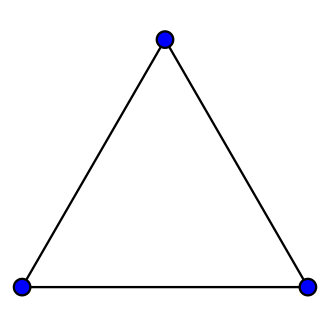
\includegraphics[width=\linewidth]
        {Figures/Complete_graph_K3.svg}
        \caption{}
    \end{subfigure}
    \hfill
    \begin{subfigure}{0.3\linewidth}
        \centering
        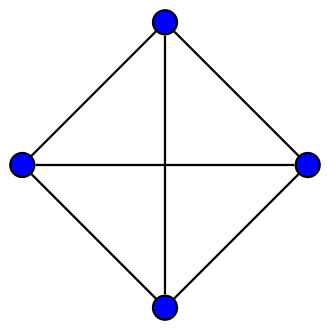
\includegraphics[width=\linewidth]
        {Figures/3-simplex_graph.svg}
        \caption{}
    \end{subfigure}
    \hfill
    \begin{subfigure}{0.3\linewidth}
        \centering
        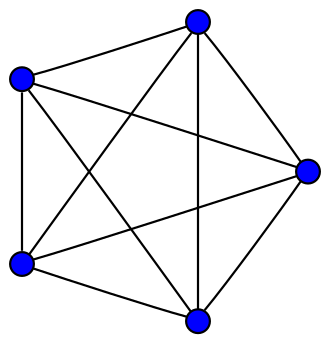
\includegraphics[width=\linewidth]{Figures/4-simplex_graph.svg}
        \caption{}
    \end{subfigure}
    
    \caption{Complete graphs.}
    \label{fig:graph}
\end{figure}


\section*{Implementation}


\subsection{Extended Kalman Filter}

Each robot estimates its own pose using an Extended Kalman Filter (EKF). This approach enables handling the nonlinear system dynamics while fusing information from multiple sensors. In particular, the EKF provides a framework to combine the internal dead-reckoning estimation with global camera-based measurements, explicitly accounting for both process and measurement uncertainties.

In our implementation, the prediction step of the EKF relies on a velocity motion model based on unicycle kinematics. The state is propagated forward using the commanded linear and angular velocities ($v$ and $\omega$) directly as control inputs. Since physical actuators are imperfect and subject to slippage or mechanical tolerances, we explicitly model this actuation uncertainty by injecting Gaussian process noise into the velocity commands. This dead-reckoning approach is effective for short-term estimation; however, it inevitably accumulates drift over time, which is subsequently corrected using the camera observations during the update step. 

The algorithm runs in two main phases at each iteration: a prediction and an update step. 

\subsubsection*{1) Prediction Step}
In this phase, the algorithm exploits the knowledge of the current state estimate and the applied control input to forecast the state at the next time step using the system's non-linear dynamics (Eq.\ref{eq:f_suv}). We have:
\begin{equation}
    \hat{s}_{k+1}^{-} = f(\hat{s}_k, u_k)
    \label{eq:ekf_predict_state}
\end{equation}
where $f$ is the model dynamics, $\hat{s}_k$ is the current state estimate, and $u_k$ is the applied control input. 

Moreover, the covariance matrix is also propagated. Since the system model is non-linear, linearization around the current estimate is required:
\begin{equation}
    P_{k+1}^{-} = A_k P_k A_k^T + G_k Q G_k^T
    \label{eq:ekf_predict_cov}
\end{equation}
with $A_k$ and $G_k$ denoting the Jacobians of the dynamics with respect to the state and the process noise at the current time step $k$, respectively:
\begin{equation}
    A_k = \left. \frac{\partial f(s, u, \nu)}{\partial s} \right|_{\substack{s=\hat{s}_k \\ u=u_k \\ \nu=0}}, \quad 
    G_k = \left. \frac{\partial f(s, u, \nu)}{\partial \nu} \right|_{\substack{s=\hat{s}_k \\ u=u_k \\ \nu=0}}
    \label{eq:ekf_jacobians}
\end{equation}
Computing explicitly the Jacobians of Eq. \ref{eq:ekf_jacobians} on the unicycle model, we obtain:
\begin{equation}
    A_k = \begin{bmatrix} 
    1 & 0 & -v_k \sin(\hat{\theta}_k)\Delta t \\ 
    0 & 1 & v_k \cos(\hat{\theta}_k)\Delta t \\ 
    0 & 0 & 1 
    \end{bmatrix}, \quad
    G_k = \begin{bmatrix} 
    \Delta t \cos(\hat{\theta}_k) & 0 \\ 
    \Delta t \sin(\hat{\theta}_k) & 0 \\ 
    0 & \Delta t 
    \end{bmatrix}
    \label{eq:ekf_matrices}
\end{equation}

\subsubsection*{2) Update Step}
Following the prediction phase, the EKF integrates the sensor measurements available at the current time step to refine the state estimate. In our framework, the sensing modality consists of a fixed global camera that provides direct observations of the robot's full pose (both 2D position and orientation). Since the sensor directly measures all the components of the state vector $\hat{s}_{k+1} = [x_{k+1}, y_{k+1}, \theta_{k+1}]^T$, the measurement model is linear. The measurement matrix $H$ is therefore the $3 \times 3$ identity matrix:
\begin{equation}
    H = \begin{bmatrix} 1 & 0 & 0 \\ 0 & 1 & 0 \\ 0 & 0 & 1 \end{bmatrix}
    \label{eq:ekf_H_matrix}
\end{equation}
Whenever a camera measurement $z_{k+1} \in \mathbb{R}^3$ becomes available at instant $k+1$, the EKF first computes the innovation:
\begin{equation}
    y_{k+1} = z_{k+1} - H \hat{s}_{k+1}^{-}
    \label{eq:ekf_innovation}
\end{equation}
Which quantifies the discrepancy between the received measurement $z_{k+1}$ and its predicted value. The covariance of the innovation is computed as:
\begin{equation}
    S_{k+1} = H P_{k+1}^{-} H^T + R_{k+1}
    \label{eq:ekf_innovation_cov}
\end{equation}
Where $R_{k+1}$ denotes the $3 \times 3$ measurement noise covariance matrix associated with the camera  (Eq.~\ref{eq:R_matr}). The Kalman gain is then evaluated as:
\begin{equation}
    W_{k+1} = P_{k+1}^{-} H^T S_{k+1}^{-1}
    \label{eq:ekf_kalman_gain}
\end{equation}
The corrected state estimate is subsequently obtained through:
\begin{equation}
    \hat{s}_{k+1} = \hat{s}_{k+1}^{-} + W_{k+1} y_{k+1}
    \label{eq:ekf_update_state}
\end{equation}
Followed by the covariance matrix update:
\begin{equation}
    P_{k+1} = (I - W_{k+1} H) P_{k+1}^{-}
    \label{eq:ekf_update_cov}
\end{equation}

This localization framework proves to be highly robust to temporary sensory loss. In scenarios where the robot is occluded by an obstacle and the global camera cannot provide a valid measurement, the system does not fail; instead, the EKF smoothly falls back on its prediction phase. State estimation is temporarily maintained via velocity-based dead-reckoning, and any accumulated drift is immediately corrected as soon as the robot re-enters the camera's field of view.



\subsection{Voronoi-Lloyd Based Partitioning}
The prerequisite of this framework is to provide a distributed control logic that works reliably and effectively in a crowded environment, enabling the swarm to explore the area, avoid obstacles, and converge around a target. For this purpose a Voronoi space partitioning was adopted, along with Lloyd-based navigation \cite{fontanelli} to converge to the target.

 Let $Q \in \mathbb{R}^2$ be the mission space, $q$ a generic point in the $Q$ space, and $p_r$ the robot position. Given the set of agents and their positions $\mathcal{P} = \{p_1, \dots, p_n\}$, the $i$-th Voronoi cell can be computed as follows:
\begin{equation}
    V_i = \{q \in Q \mid \|q - p_i\| \leq \|q - p_j\|, \forall j \neq i\}
    \label{eq:voronoi_cell}
\end{equation}
Equation \ref{eq:voronoi_cell} assigns each robot located at $p_i$ a portion of the map: its Voronoi cell $V_i$. This region contains all points that are closer to robot $i$ than to all other robots, intrinsically granting inter-robot collision avoidance.
\\

The Voronoi partitioning alone does not prevent collisions with static obstacles. To enforce this, the cell $V_i$ is constrained by the robot's sensing radius $r_s$ and line-of-sight visibility.


We define the $i$-th visibility set $S_i$ using a ray-casting approach, where the line-of-sight is interrupted if it intersects an obstacle:
\begin{equation}
    S_i = \{q \in V_i \mid p_i - \gamma(p_i - q) \notin \mathcal{O}\}, \ \  \forall \gamma \in [0,1]
\end{equation}
Where $\mathcal{O} \subset Q$ is the obstacle set, i.e., the set of points in the map corresponding to static obstacles.


At this point, the resulting visibility set $S_i$ is intersected with the Voronoi cell, reducing it to the intermediate set $\bar{W_i}= V_i \cap S_i$. The reduced cell $\bar{W_i}$ is then bounded by the physical sensing radius of the robot $r_s$, yielding the final safe navigation cell $W_{i}$:
\begin{equation}
    W_{i} = \{q \in\bar{W_i} \mid \|q - p_r\| \leq r_s\}
    \label{eq:trimmed_cell}
\end{equation}

In practice, the visibility set and sensing limit $r_s$ are computed simultaneously using a ray-casting algorithm  similar to what presented in \cite{raycast} implemented via the Python \texttt{Shapely} library.

Radial rays, spaced by the angular resolution set by the LiDAR, are cast from the robot up to a distance $r_s$ and geometrically truncated at the exact point of intersection with any obstacle.Connecting the endpoints of these rays creates a strictly bounded visibility polygon, $S_i$. The final safe navigation cell $W_{i}$ is then efficiently obtained through a geometric boolean intersection:
\begin{equation}
    W_{r_s} = V_i \cap S_i
    \label{eq:final_safe_cell}
\end{equation}

To accurately simulate the characteristics of a real LiDAR sensor, noise is injected into the computed ray lengths, as described in Eq. \ref{eq:lidar_noise}.

Another aspect to consider is that each agent requires the positions of its peers to compute its local Voronoi cell. To achieve this, every robot periodically shares its estimated position with the rest of the swarm via the previously described broadcast mechanism. This approach introduces an important layer of realism to the simulation, as the robots do not possess instantaneous, continuous knowledge of each other's true states. Instead, the spatial partitioning relies entirely on the last known positions received from the network, accurately reflecting the discrete nature of real-world communication systems.

The outcome of this decentralized partitioning is illustrated in Fig. \ref{fig:vor}. As can be observed, the boundaries of the resulting Voronoi cells are not perfectly smooth, which is a direct consequence of the simulated LiDAR measurement noise. Furthermore, the spatial separation between the robots is slightly asymmetrical; this reflects the communication delays, as each agent computes its cell based on the periodically broadcasted, and therefore slightly outdated, positions of its peers.

\begin{figure}[H]
    \centering
    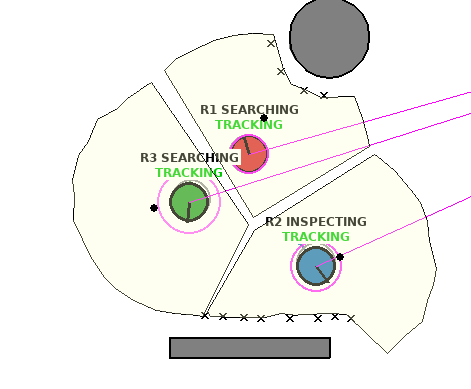
\includegraphics[width=0.6\linewidth]{Figures/voronoi.png}
    \caption{Voronoi partition.}
    \label{fig:vor}
\end{figure}




\subsection{Control FSM}
To govern the behavior of the agents according to their current objectives, a Finite State Machine (FSM) was developed. Before detailing the specific states and transitions of the FSM, we first mathematically formulate the underlying control laws that dictate the robots' kinematics ($[v, \omega]^T$) in various scenarios: exploration, obstacle avoidance, boundary mapping, and target formation.

\subsubsection*{1) Lévy Flight Control}
During the search phase, pure random walks are highly inefficient. Instead, the robots employ a Lévy flight exploration strategy. This method mimics the optimal foraging behaviors naturally observed in the animal kingdom, such as those of marine predators searching for prey \cite{levyDISTRIB}. Taking inspiration from the framework presented in \cite{levyUSED}, a new target heading $\theta_{target}$ is chosen uniformly at random, while the duration for which the robot maintains this heading is periodically sampled from a stable Lévy distribution, as illustrated in Fig. \ref{fig:levy}. 

\begin{figure}[H]
    \centering
    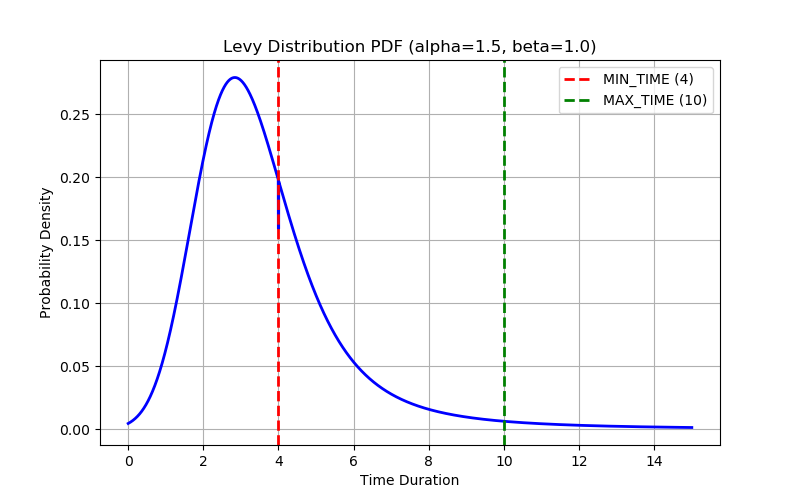
\includegraphics[width=0.65\linewidth]{Figures/Levy_distrib.png}
    \caption{Lévy distribution used.}
    \label{fig:levy}
\end{figure}

To ensure practical applicability, minimum and maximum temporal bounds are enforced on the sampled values, which are also reported in the figure. These boundaries and the distribution parameters can be easily fine-tuned to better suit the scale and specific requirements of the mission at hand. This time-based sampling generates a characteristic movement pattern consisting of many short, localized searches interspersed with occasional long-distance relocations, allowing the swarm to cover large areas efficiently. 
So during a time interval a vector $\vec{v}_{levy}$ is generated as:
\begin{equation}
   \vec{v}_{levy} = \begin{bmatrix} \cos \theta_{target} \\ \sin \theta_{target} \end{bmatrix}
   \label{eq:levy_vecotor}
\end{equation}





\subsubsection*{2) Obstacle Avoidance Control}
To prevent collisions during exploration, a repulsive approach is adopted through a quadratic bounded repulsive force. 

Let $d = \|p - p_{vor}\|$ be the Euclidean distance from the robot's position $p$ to the closest point $p_{vor}$ on its Voronoi. If this distance falls below a critical safety threshold $d_{min}$, a repulsive vector $\vec{v}_{rep}$ is generated:

\begin{equation}
\vec{v}_{rep} = 
\begin{cases} 
k_{rep} (d_{min} - d)^2 \frac{p - p_{obs}}{d} & \text{if } d < d_{min} \\ 
\mathbf{0} & \text{if } d \geq d_{min} 
\end{cases}
\label{eq:repuls_vect}
\end{equation}

Where $k_{rep}$ is the repulsive gain. The fraction $\frac{p - p_{obs}}{d}$ computes the normalized directional vector pointing away from the obstacle. 


\subsubsection*{3) Wall Following Control}
When a robot encounters an obstacle, it enters an inspection phase to map its perimeter. To do so, this controller makes the robot slide along the obstacle's boundary. To achieve a smooth sliding behavior while maintaining a safe distance, the control vector is computed as the superposition of a tangential component along the boundary and a normal distance correction.

Let $\vec{n}$ be the normalized vector pointing from the robot's position $p$ to the closest point on its Voronoi cell boundary (which represents the closest obstacle), $p_{obs}$, defined as $\vec{n} = \frac{p_{obs} - p}{\|p_{obs} - p\|}$. A tangent vector $\vec{t}$ is derived by rotating $\vec{n}$ by 90 degrees: $\vec{t} = [-m_{dir} n_y, m_{dir} n_x]^T$, where $m_{dir} \in \{1, -1\}$ dictates the sliding direction (counter-clockwise or clockwise). This direction is chosen randomly whenever a new obstacle is encountered. 

To ensure the robot does not drift away or crash, a proportional controller corrects the distance error $e = \|p_{obs} - p\| - d_{target}$, where $d_{target}$ is the desired safe distance from the wall. The desired movement vector is thus formulated as:

\begin{equation}
\vec{v}_{des} = 
\begin{bmatrix} 
v_{des,x} \\ 
v_{des,y} 
\end{bmatrix}
= \vec{t} + K_p \cdot e \cdot \vec{n}
\end{equation}

Where $K_p$ is the proportional gain. 

The robot aligns its motion with this vector's angle, $\theta_{target} = \arctan2(v_{des,y}, v_{des,x})$, utilizing the following control law:

\begin{equation}
u_{wall} = 
\begin{bmatrix} 
v \\ 
\omega 
\end{bmatrix}
=
\begin{bmatrix} 
V_{lin} \cos^3(\theta_{target} - \theta)) \\ 
K_\omega (\theta_{target} - \theta) 
\end{bmatrix}
\label{eq:wall_follow_control}
\end{equation}

Where $V_{lin}$ is the maximum linear velocity, $K_\omega$ is the angular velocity gain, and $\theta$ is the current heading of the robot.

Notably, the linear velocity is modulated by the cubed cosine of the heading error ($\cos^3$). This ensures a highly responsive behavior: if the angle error is large, the forward speed drops dramatically, allowing the robot to perform tight corrective turns before resuming its sliding motion along the wall.


\subsubsection*{4) Formation Control and Lloyd's Algorithm}
Once the target is located, the swarm transitions from exploration to a coordinated formation phase. To achieve a stable and distributed configuration around the target, the Voronoi-based coverage strategy known as Lloyd's Algorithm is employed \cite{fontanelli, Loyd_usato} and modified to incorporate environmental constraints and a specific spatial density.

The fundamental objective is to distribute the agents according to a desired spatial density, defined by a Probability Density Function $\phi(q)$. Our framework follows the approach presented in \cite{Loyd_usato}, where $\phi(q)$ is designed as a ring-shaped PDF (Fig.\ref{fig:ringPDF}) centered at the estimated target position $p_{target}$. Specifically, this distribution is defined as:

\begin{equation}
    \phi(q) = \exp \left( -\frac{(\|q - p_{target}\| - R_{ring})^2}{2\sigma^2} \right)
\end{equation}

Where $q$ is a generic point in the mission space $Q$ and $R_{ring}$ is the desired radius of the circular formation. If $R_{ring} = 0$, the distribution collapses to a standard Gaussian centered on the target. To improve stability and prevent oscillations when agents are far from the goal, an adaptive standard deviation $\sigma$ is used:
\begin{equation}
    \sigma = \sigma_0 \left( 1 + \frac{\|p - p_{target}\|}{R_{ad}} \right)
\end{equation}
Where $\sigma_0$ is the base spread and $R_{ad}$ is a scaling distance. 

\begin{figure}[H]
    \centering
    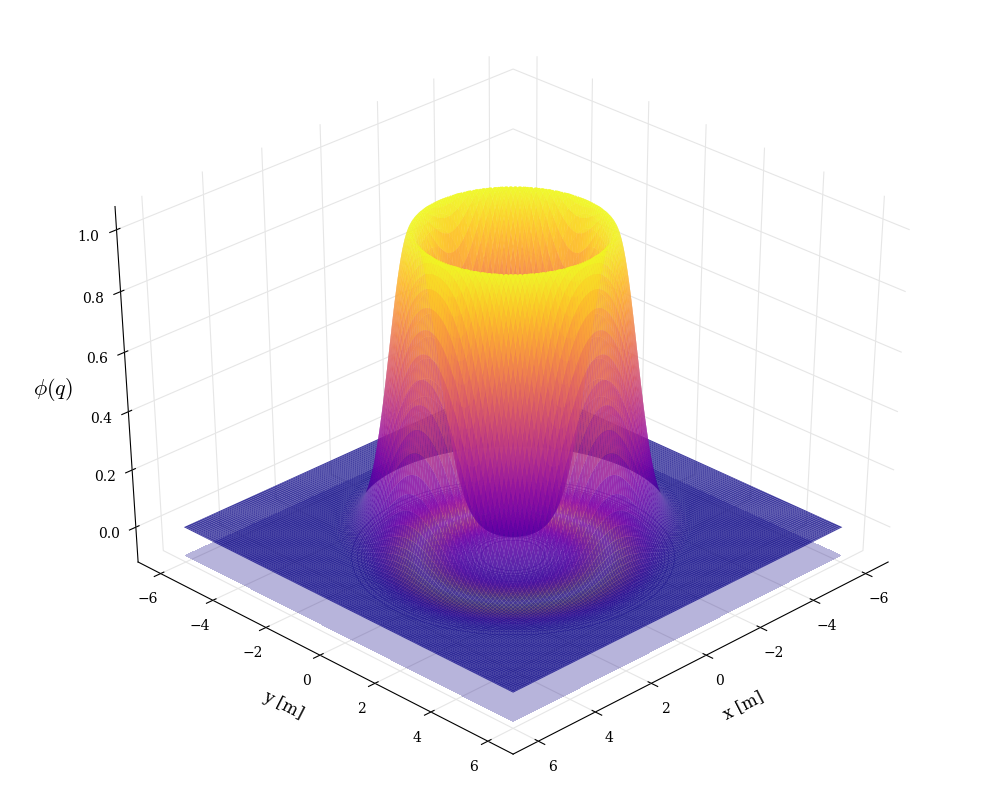
\includegraphics[width=0.6\linewidth]{Figures/ring_PDF.png}
    \caption{Ring shaped PDF}
    \label{fig:ringPDF}
\end{figure}

For each agent $i$, we compute the "mass" $M_{V_i}$ and the weighted centroid $C_{V_i}$ of its Voronoi cell $V_i$ as:
\begin{equation}
    M_{V_i} = \int_{V_i} \phi(q) \, dq, \quad C_{V_i} = \frac{1}{M_{V_i}} \int_{V_i} q \phi(q) \, dq
\end{equation}
The centroid $C_{V_i}$ represents the local optimal position. Thus, we can define the Lloyd-based target vector as follows:
\begin{equation}
    \vec{v}_{target} =  \begin{bmatrix} v_{target,x} \\ v_{target,y} \end{bmatrix}= (C_{V_i} - p) + k_{rep} \cdot \vec{v}_{rep}
\end{equation}
Where $\vec{v}_{rep}$ is the repulsive vector from nearby obstacles. While the standard Lloyd control is inherently robust, the addition of the repulsive term ensures an extra layer of safety, allowing the robots to navigate more reliably around obstacles during the formation process.

Finally, the robot's velocities are generated using the following control law:
\begin{equation}
    u_{lloyd} = \begin{bmatrix} v \\ \omega \end{bmatrix} = \begin{bmatrix} V_{lin} \ \cos^3(\theta_{target} - \theta) \\ K_\omega (\theta_{target} - \theta) \end{bmatrix}
    \label{eq:lloyd_control}
\end{equation}
Where $\theta_{target} = \arctan2(v_{target,y}, v_{target,x})$. This formulation allows the swarm to converge smoothly into a ring formation while maintaining safety distances from boundaries.
\\


With the underlying control laws mathematically defined, we can now detail the Finite State Machine (FSM) that dictates the high-level behavior of each agent. The FSM is designed to seamlessly manage the transitions between exploration, obstacle mapping, and target formation. It consists of three primary states:

\subsubsection*{1) Searching}
This is the default exploration state. In this phase, the agent navigates the environment using the Lévy flight exploration strategy. To ensure safe navigation, the desired Lévy direction is continuously superimposed with the obstacle avoidance control vector. The resulting direction vector is thus defined as the combination of Eq.\ref{eq:levy_vecotor} and Eq.\ref{eq:repuls_vect}:
\begin{equation}
    \vec{v}_{search} = \begin{bmatrix} v_{search,x} \\ v_{search,y} \end{bmatrix} = \vec{v}_{levy} + \vec{v}_{rep}
\end{equation}

From this combined vector, the new target heading is computed using the four-quadrant inverse tangent:
\begin{equation}
    \theta_{target} = \text{arctan2}(v_{search,y}, v_{search,x})
\end{equation}

To prevent the robot from moving forward while correcting large angular deviations—which could lead to unsafe behaviors near obstacles—a piecewise control law is applied to the linear velocity, while the angular velocity remains proportional to the error:
\begin{equation}
    u_{search} = \begin{bmatrix} v \\ \omega \end{bmatrix} = 
    \begin{bmatrix} 
        \begin{cases} 
            0 & \text{if } |e_\theta| > \frac{\pi}{4} \\ 
            V_{lin} \cos(e_\theta) & \text{otherwise} 
        \end{cases} \\ 
        K_\omega \, e_\theta 
    \end{bmatrix}
\end{equation}

Where $e_\theta = (\theta_{target} - \theta)$ is the angular error.
This control strategy allows the robot to rotate in place when a sharp turn is required (e.g., when suddenly repelled by a boundary), and perform smooth, modulated (by the cosine) curves otherwise. The robot continues this exploratory behavior until its simulated LiDAR detects a physical obstacle within a predefined distance threshold. If the detected obstacle points have not been previously mapped by the swarm, the FSM transitions the robot to the \texttt{INSPECTING} phase.

\subsubsection*{2) Inspecting}
Upon encountering an unmapped obstacle, the robot temporarily suspends random exploration and enters the \texttt{INSPECTING} state. Here, the FSM switches to the wall-following control strategy $u_{wall}$ (Eq.\ref{eq:wall_follow_control}). The agent slides along the contour of the obstacle at a safe distance $d_{target}$, collecting new boundary points and continuously updating the swarm's shared map. 


The robot reverts to the \texttt{SEARCHING} state under three specific conditions: if it detects a loop closure (indicating it has fully circumnavigated the obstacle or merged with an already mapped area), if it reaches a critical proximity to another robot (triggering a collision avoidance maneuver), or if it simply loses track of the wall.

\subsubsection*{3) Treasure Found}
This terminal phase is activated when the robot either enters the physical sensing range of the target object or receives the target's estimated coordinates through the swarm's consensus network. Once activated, both exploration and mapping halt entirely, and the FSM delegates the kinematic commands to the Voronoi-based Formation Control, $u_{lloyd}$ (Eq.\ref{eq:lloyd_control}). In this state, the agent converges toward the target and begins to arrange itself into the ring formation. While maintaining this formation, the robot continuously computes a weighted average of the target's position to build a shared consensus estimate, maneuvering to distribute itself evenly along the desired circular formation defined by the ring-shaped probability density function.



\subsection{Collaborative Mapping}
The mapping process begins with measurements acquisition through the LiDAR sensor. For each agent, a raycasting algorithm is executed in the same way as described in the Voronoi discussion \cite{raycast}. These intersections yield a set of local measurements $z_d$ (Eq.\ref{eq:lidar_noise}) and their relative angle $ \alpha$, representing the range and bearing of the detected points relative to the robot's sensor frame.

It is worth highlighting the realistic nature of the mapping mechanism employed to process these raw readings. In real-world applications, a robot perceives the environment relative to its true physical location, but it must register these sensor readings in a global coordinate frame relying solely on its estimated state. To faithfully replicate this paradigm, the simulated LiDAR captures measurements originating from the robot's ground-truth state, defined as $\mathbf{s} = [x, y, \theta]^T$. 

However, because $\mathbf{s}$ is unknown to the robot, the mapping algorithm intentionally integrates the physical measurements $(z_d, \alpha)$ exclusively with the robot's current state estimate provided by the Extended Kalman Filter (EKF), denoted as $\hat{s} = [\hat{x}, \hat{y}, \hat{\theta}]^T$. To compute the absolute global coordinates of the newly discovered boundary points, $p_{map}$, a rigid body transformation is applied using the estimated state:
\begin{equation}\begin{split}
    p_{map} & = \begin{bmatrix} \hat{x} \\ \hat{y} \end{bmatrix} + \begin{bmatrix} \cos(\hat{\theta}) & -\sin(\hat{\theta}) \\ \sin(\hat{\theta}) & \cos(\hat{\theta}) \end{bmatrix} \begin{bmatrix} z_d \cos(\alpha) \\ z_d \sin(\alpha) \end{bmatrix}\\
    & = \begin{bmatrix} \hat{x} + z_d \cos(\hat{\theta} + \alpha) \\ \hat{y} + z_d \sin(\hat{\theta} + \alpha) \end{bmatrix}
\end{split}\end{equation}

As a result, the computed points $p_{map}$ are affected by the estimation error $e = x_{true} - \hat{x}_{ekf}$. The constructed shared map inherently reflects the localization uncertainties of the swarm, accurately modeling the intrinsic challenges of real-world robotic mapping where odometry drift directly distorts the generated map.

Furthermore, the shared map is distributed across the swarm as a component of the broadcasted communication payload. Consequently, the global map is not instantaneously synchronized across the memory of all agents. Instead, newly mapped boundary points propagate iteratively through the network as the robots exchange data. This delayed, decentralized synchronization further enhances the realism of the simulation, accurately reflecting the communication constraints and data propagation dynamics inherent to physical multi-robot systems.


\subsection{Consensus}
Once the target is detected, the objective of the swarm is to accurately estimate its true position $p_{target}$ despite the presence of significant LiDAR sensor noise (Eq.\ref{eq:lidar_noise}) and also taking into account the fact that the agents communicate one at a time. To achieve this, the proposed framework implements the broadcast gossip algorithm discussed in \cite{consensusUSATO} alongside a two-tier estimation strategy: a temporal local sensor fusion (intra-robot) and a spatial network consensus (inter-robot). Crucially, both mechanisms continuously update the same variable, denoted as $\hat{p}_i$ for the $i$-th robot.

\subsubsection*{1) Local Temporal Fusion}
When an agent is within the physical sensing range of the target, it periodically samples the treasure at 1 Hz, obtaining a noisy measurement $z_{treasure}$ at fixed time intervals. Instead of relying on a single raw reading or storing large arrays of past measurements, the robot maintains a running average using a dynamic learning rate $\alpha$. Let $N_i$ be the total number of measurements taken by the $i$-th robot. The weight is defined as:

\begin{equation}
    \alpha = \frac{1}{N_i}
\end{equation}

The local value $\hat{p}_i$ is then iteratively updated as:

\begin{equation}
    \hat{p}_i^+ = (1-\alpha)\hat{p}_i^- + \alpha z_{treasure}
    \label{eq:temporal_filter}
\end{equation}

This formulation corresponds to the exact mathematical average of all local measurements. As $N_i$ increases over time, $\alpha$ approaches zero, effectively filtering out the zero-mean Gaussian noise (Eq.\ref{eq:lidar_noise}) and stabilizing the local estimate.

\subsubsection*{2) Spatial Network Consensus}
To propagate this knowledge across the swarm, the agents utilize the Broadcast Gossip algorithm introduced next. When robot $i$ receives a payload containing a target estimate $\hat{p}_j$ from robot $j$, it fuses this incoming data directly into its own current state $\hat{p}_i$. The update law is governed by a constant mixing parameter $\gamma \in (0,1)$:

\begin{equation}
    \hat{p}_i^+ = (1-\gamma)\hat{p}_i^- + \gamma \hat{p}_j
    \label{eq:spatial_filter}
\end{equation}

In our implementation, $\gamma$ is set to $0.5$, which computes the exact midpoint between the two estimates. Because both the temporal sensor fusion and the network gossip updates the exact same variable $\hat{p}_i$, a continuous distributed filter is inherently created. The discovering agents act as anchors, pulling their state toward the physical measurements, while this pairwise averaging rapidly drives the rest of the swarm to agree on a highly accurate global estimate, mitigating any residual local biases.

\paragraph{Mathematical Formalization of Broadcast Gossip Consensus}
Suppose that at time instant $k$, node $i$ is designated to share its estimate with the other agents. In this case, the remaining $N - 1$ robots, assuming no communication losses, receive the broadcasted value $\hat{p}_i(k)$ and update their spatial estimate as:
\begin{equation}
    \hat{p}_j(k+1) = \gamma \hat{p}_i(k) + (1-\gamma)\hat{p}_j(k), \quad \forall j \neq i,
\end{equation}
while the broadcaster keeps its current estimate:
\begin{equation}
    \hat{p}_i(k+1) = \hat{p}_i(k).
\end{equation}

These equations can be written compactly in vector form as:
\begin{equation}
    \mathbf{\hat{p}}(k+1) = Q(k)\mathbf{\hat{p}}(k)
\end{equation}
where $\mathbf{\hat{p}}(k) = [\hat{p}_1(k), \dots, \hat{p}_N(k)]^T \in \mathbb{R}^N$ is the global state vector containing the estimates of all robots, and the entries of the stochastic update matrix $Q(k) \in \mathbb{R}^{N \times N}$, corresponding to a broadcast by node $i$, are given by:
\begin{equation}
    Q_{lm} = 
    \begin{cases} 
        1, & l = m = i \\ 
        1 - \gamma, & l = m \neq i \\ 
        \gamma, & m = i, \ l \neq i \\ 
        0, & \text{otherwise} 
    \end{cases}
\end{equation}

This matrix is inherently \textit{row-stochastic} (each row sums to 1), which guarantees that the system remains mathematically stable. In our specific implementation, setting $\gamma = 0.5$ forces the receiving nodes to compute the exact arithmetic mean between their own estimate and the received one.

The $Q$ matrix being row-stochastic, rather than doubly stochastic, only guarantees the convergence of the robot estimates to a consensus value, not to the exact average of their initial states (as demonstrated in \cite{consensusUSATO}). However, in our framework, computing a static average is not the objective; the goal is to find the exact physical location of the target. To overcome the theoretical limitations of a purely row-stochastic matrix, we leverage the Local Temporal Fusion described previously. 

Because both the temporal sensor fusion (Eq.\ref{eq:temporal_filter}) and the spatial network consensus (Eq.\ref{eq:spatial_filter}) sequentially update the exact same state variable $\hat{p}_i$, they create a deeply intertwined distributed filter. 

When a discovering robot updates its estimate with a new LiDAR measurement, it injects physical reality into its estimate. When it subsequently broadcasts this estimate, the receiving robots mix this physically-grounded estimate with their own. Therefore, the "current estimate" of any robot at time $k$ is actually a continuous accumulation of its own past measurements deeply mixed with the measurements of other robots shared via the network. As can be seen in Fig.\ref{fig:grafico_errore}, with this framework the estimation error converges to zero.



\section*{Statistical Analysis and Validation}
\begin{table}[htbp]
    \centering
    \renewcommand{\arraystretch}{1.2} 
    \begin{tabular}{@{}llc@{}}
        \toprule
        \textbf{Parameter} & \textbf{Value} & \textbf{Unit} \\
        \midrule
        Sensing Range ($r_s$) & 3.0 & m \\
        Nominal Linear Velocity ($V_{lin}$) & 1.0 & m/s \\
        Obstacle Avoidance Threshold ($d_{min}$) & 1.0 & m \\
        Angoular Velocity Gain ($K_\omega$) ($\alpha$) & 1 & - \\
        Repulsive Gain Exploration ($k_{rep}$) & 8.0 & - \\
        Repulsive Gain Formation ($k_{rep}$) & 0.5 & - \\
        Ray-Casting Resolution & 10.0 & deg \\
        Velocity Noise Std Dev ($\sigma_v$) & 0.05 & m/s \\
        Angular Vel. Noise Std Dev ($\sigma_\omega$) & 0.01 & rad/s \\
        Camera X-Pos. Noise Std Dev ($\sigma_x$) & 0.1 & m \\
        Camera Y-Pos. Noise Std Dev ($\sigma_y$) & 0.1 & m \\
        Camera Heading Noise Std Dev ($\sigma_\theta$) & 0.05 & rad \\
        LiDAR Noise Std Dev ($\sigma_d$) & 0.05 & m \\
        \bottomrule
    \end{tabular}
    \caption{Simulation and Control Parameters}
    \label{tab:sim_parameters}
\end{table}


To rigorously evaluate the performance and robustness of the proposed multi-agent framework, a statistical analysis was conducted. Relying on a single simulation run is insufficient to assess systems heavily influenced by stochastic processes, such as Lévy flight exploration, LiDAR measurement noise, and communication dynamics. Therefore, $100$ independent simulations were executed in a fully decentralized, parallelized environment. Each run was allowed a maximum simulated time of $600$ seconds, which provided ample time for the swarm to explore the environment, detect the target, and achieve formation.

The statistical evaluation focused on three primary indicators:

\subsubsection*{1) Map coverage}
Since the explorative movement of the agent is determined by the Lévy flight controller, we need to evaluate its efficiency in the map coverage. During the 100 simulations, the path taken by each robot has been recorded and displayed. By analyzing the result reported in Figure \ref{fig:grafico_traiettorie}, one can discover controller patterns or find blind areas, which would underline a failure in the map exploration task.

\begin{figure}[H]
    \centering
    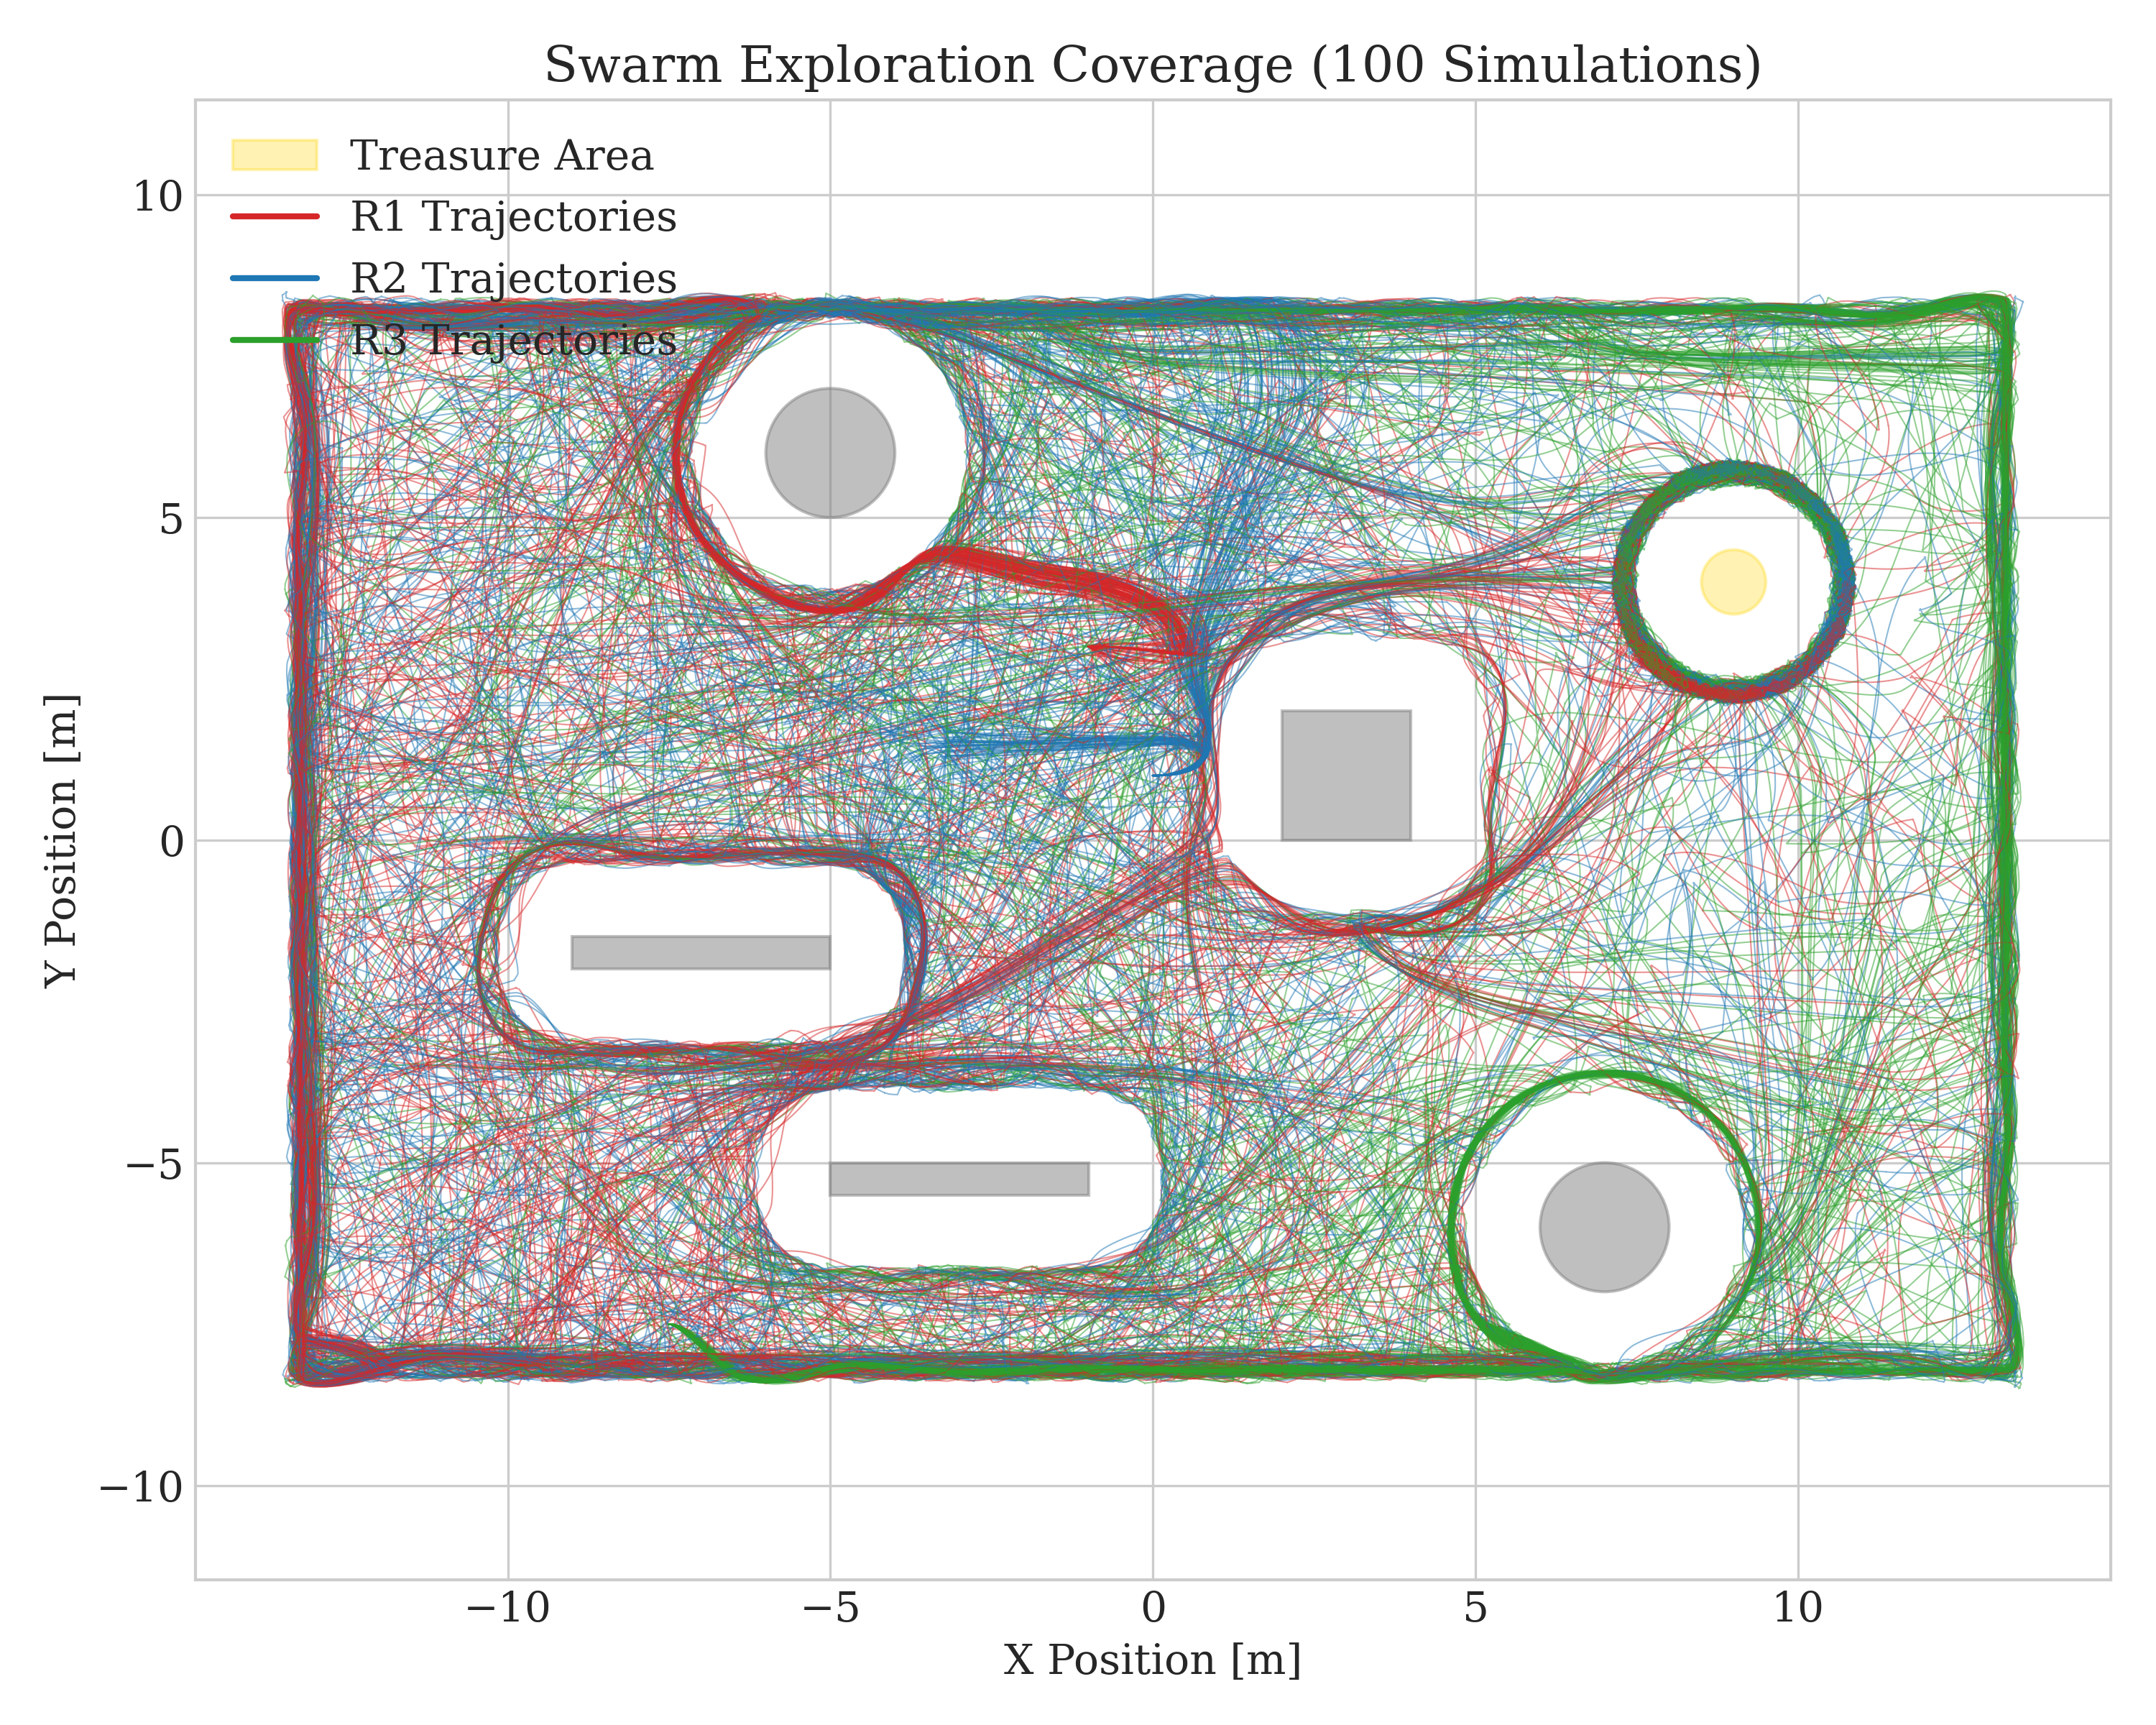
\includegraphics[width=0.8\linewidth]{Figures/grafico_traiettorie.png}
    \caption{Map exploration coverage}
    \label{fig:grafico_traiettorie}
\end{figure}

Observation of interesting behaviors about the controller implemented in the project is possible by focusing on Figure \ref{fig:grafico_traiettorie}: 

\begin{itemize}[noitemsep]
    \item The external walls are heavily traced, meaning the robots have a tendency to run along it, rather than wandering around the room.
    
    \item The entirety of the map seems to have pretty much the same coverage density. The only parts which are less explored are the bottom-right part, which is the farthest point from the robots' starting position, and the area around the treasure.
\end{itemize}

With this analysis, the Lévy flight control has been demonstrated, as expected, to be effective and thus is appropriate for this kind of application.

\subsubsection*{2) Target Estimation Convergence}
To evaluate the effectiveness of the two-tier sensor fusion and consensus algorithms, the global estimation error was tracked over time. The error is defined as the Euclidean distance between the true target position $p_{target}$ and the swarm's average estimated position $\hat{p}_{avg}(t)$ at any given time step $t$.To ensure a consistent comparison across all $100$ runs, the observation window was synchronized to start at $t=0$, defined as the exact moment the first robot physically detects the target. Figure \ref{fig:grafico_errore} illustrates the mean estimation error of the swarm over a $50$-second observation window following the initial detection. The solid blue line represents the mean error, while the shaded region denotes the standard deviation bounds ($\pm 1\sigma$).

\begin{figure}[H]
    \centering
    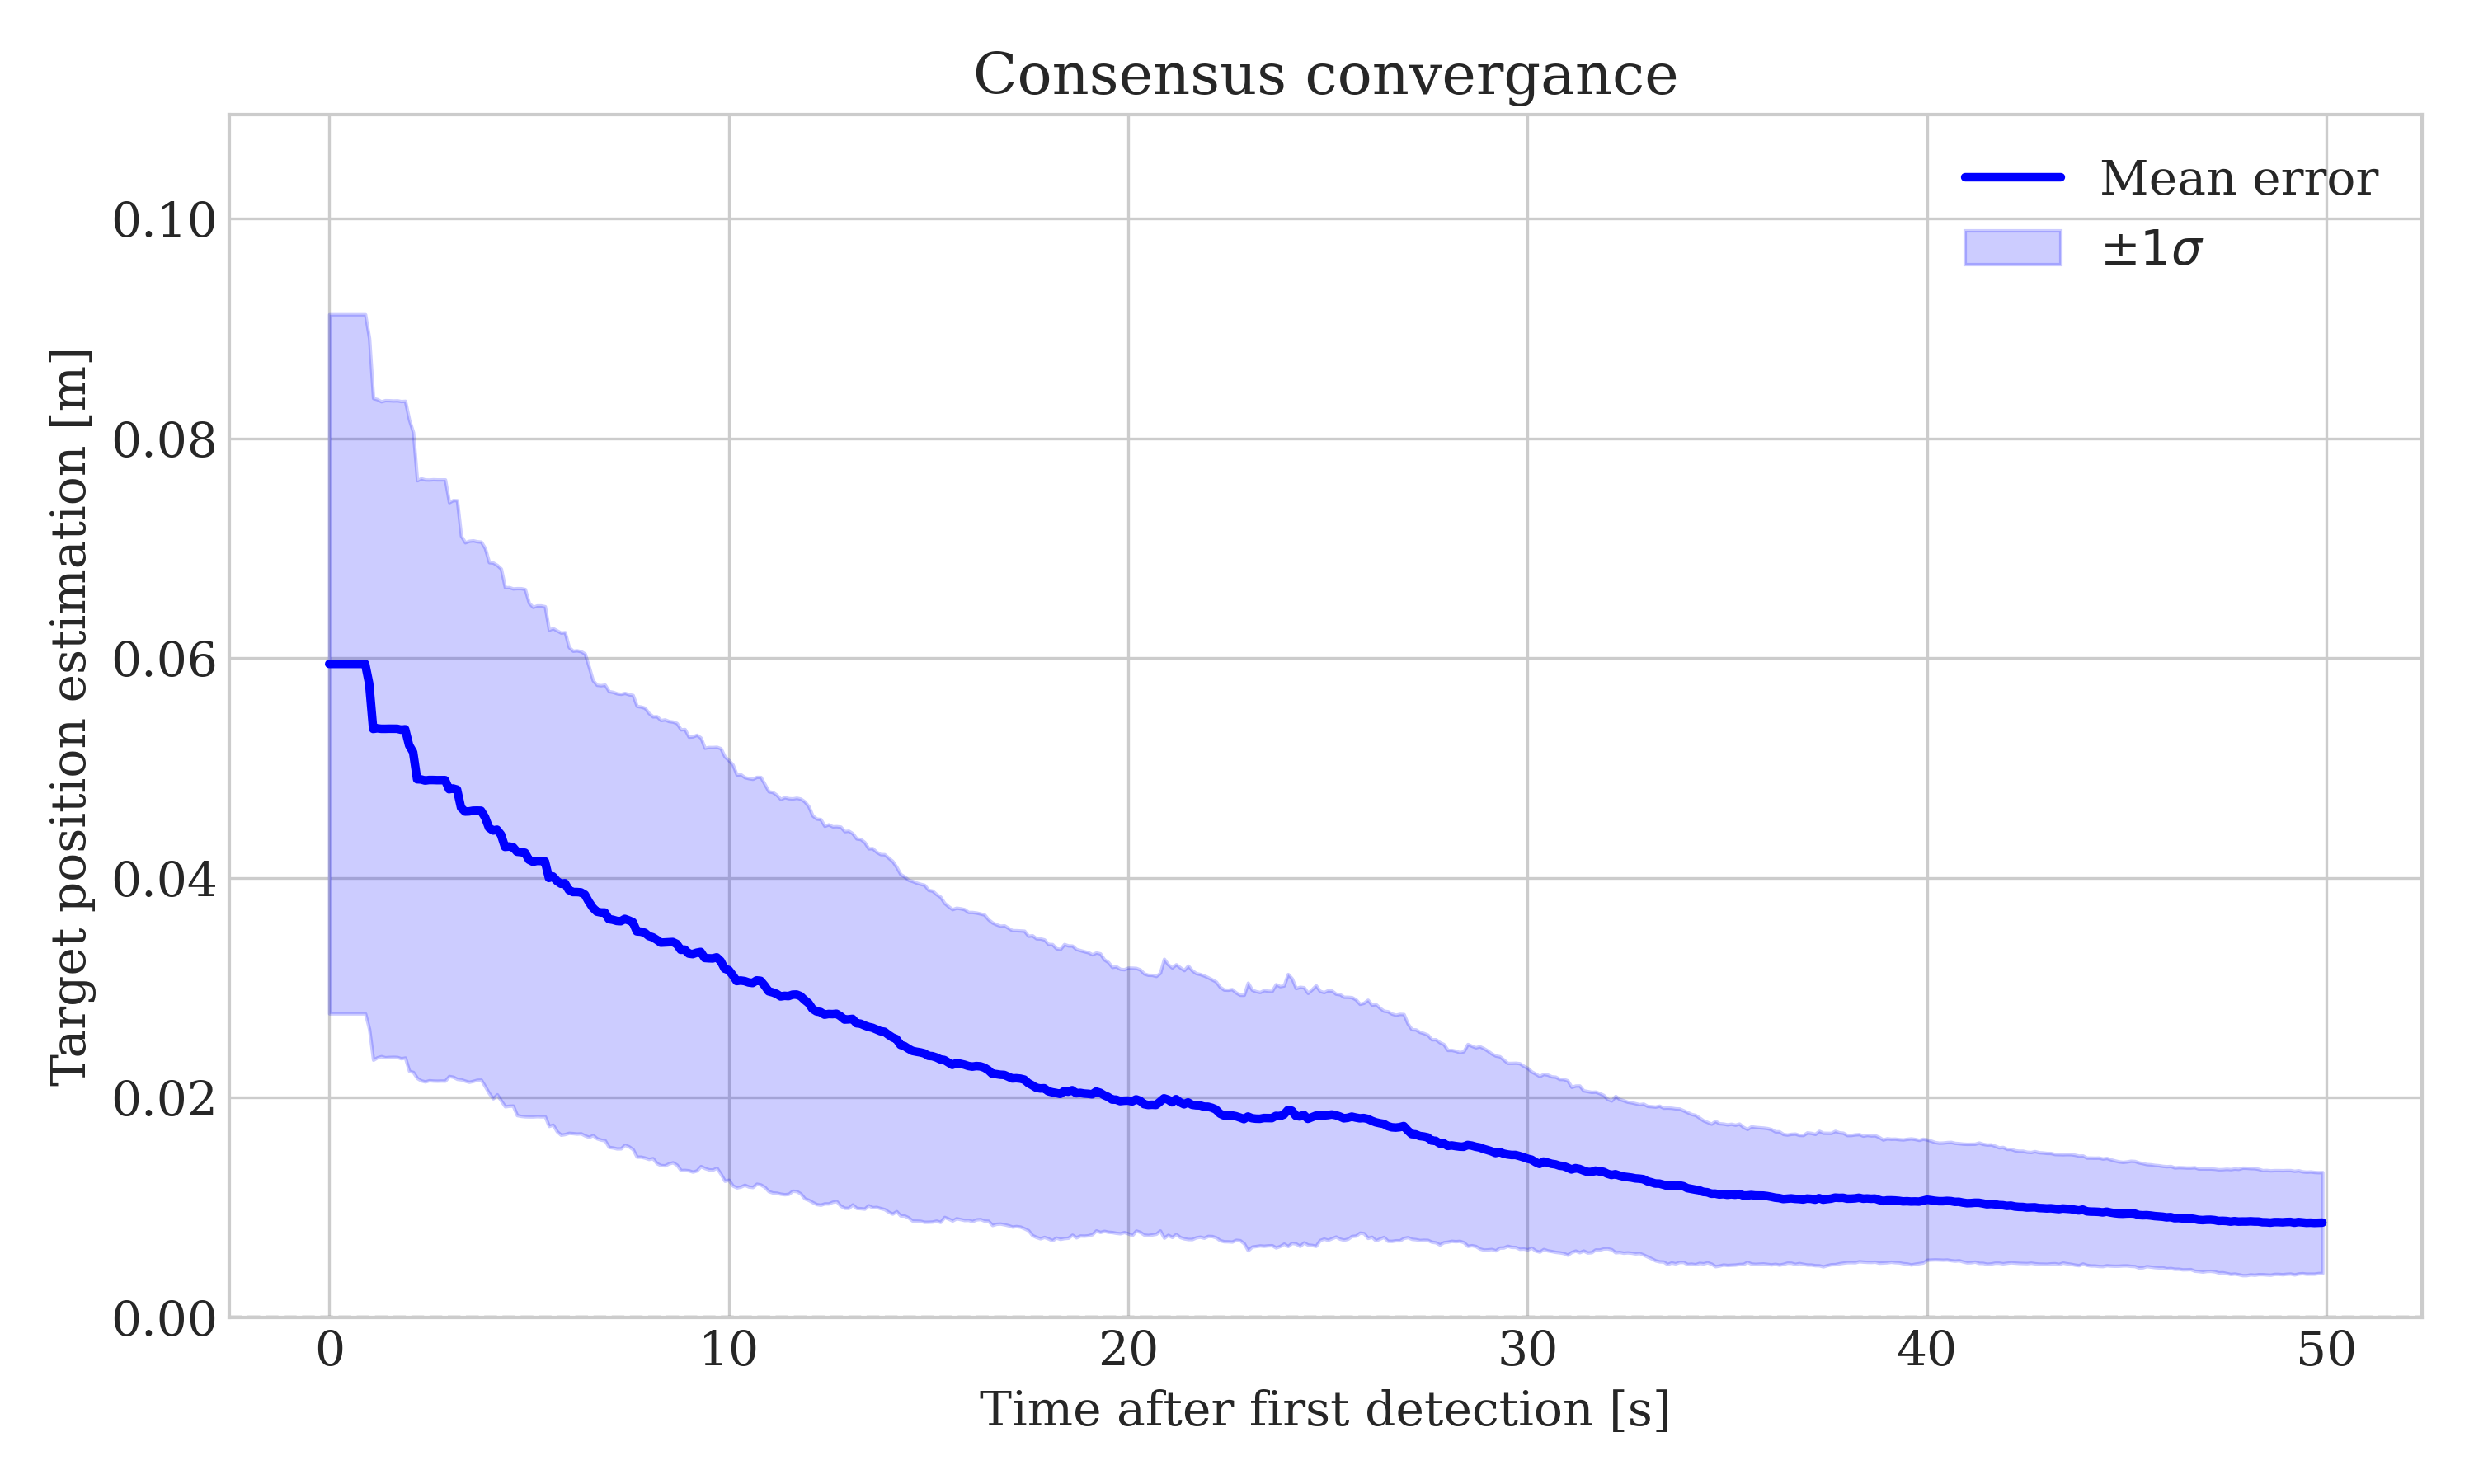
\includegraphics[width=0.8\linewidth]{Figures/grafico_errore.png}
    \caption{Target estimation error}
    \label{fig:grafico_errore}
\end{figure}

The plot clearly demonstrates the power of the consensus algorithm: the initial estimation error drops precipitously as the first agent refines its local measurement using the temporal filter (Eq. \ref{eq:temporal_filter}). Furthermore, as the second and third robots arrive at the target and inject their independent readings into the broadcast network, the global error asymptotically converges toward zero, while the variance narrows significantly. This proves that the swarm's collective intelligence successfully mitigates individual sensor noise.

\subsubsection*{3) Spatial Coordination and Arrival Efficiency}
The second metric evaluates the efficiency of the exploration by recording the exact time it took for the first (FTT), second (STT), and third (TTT) robot to physically reach the target sensing radius.

\begin{figure}[H]
    \centering
    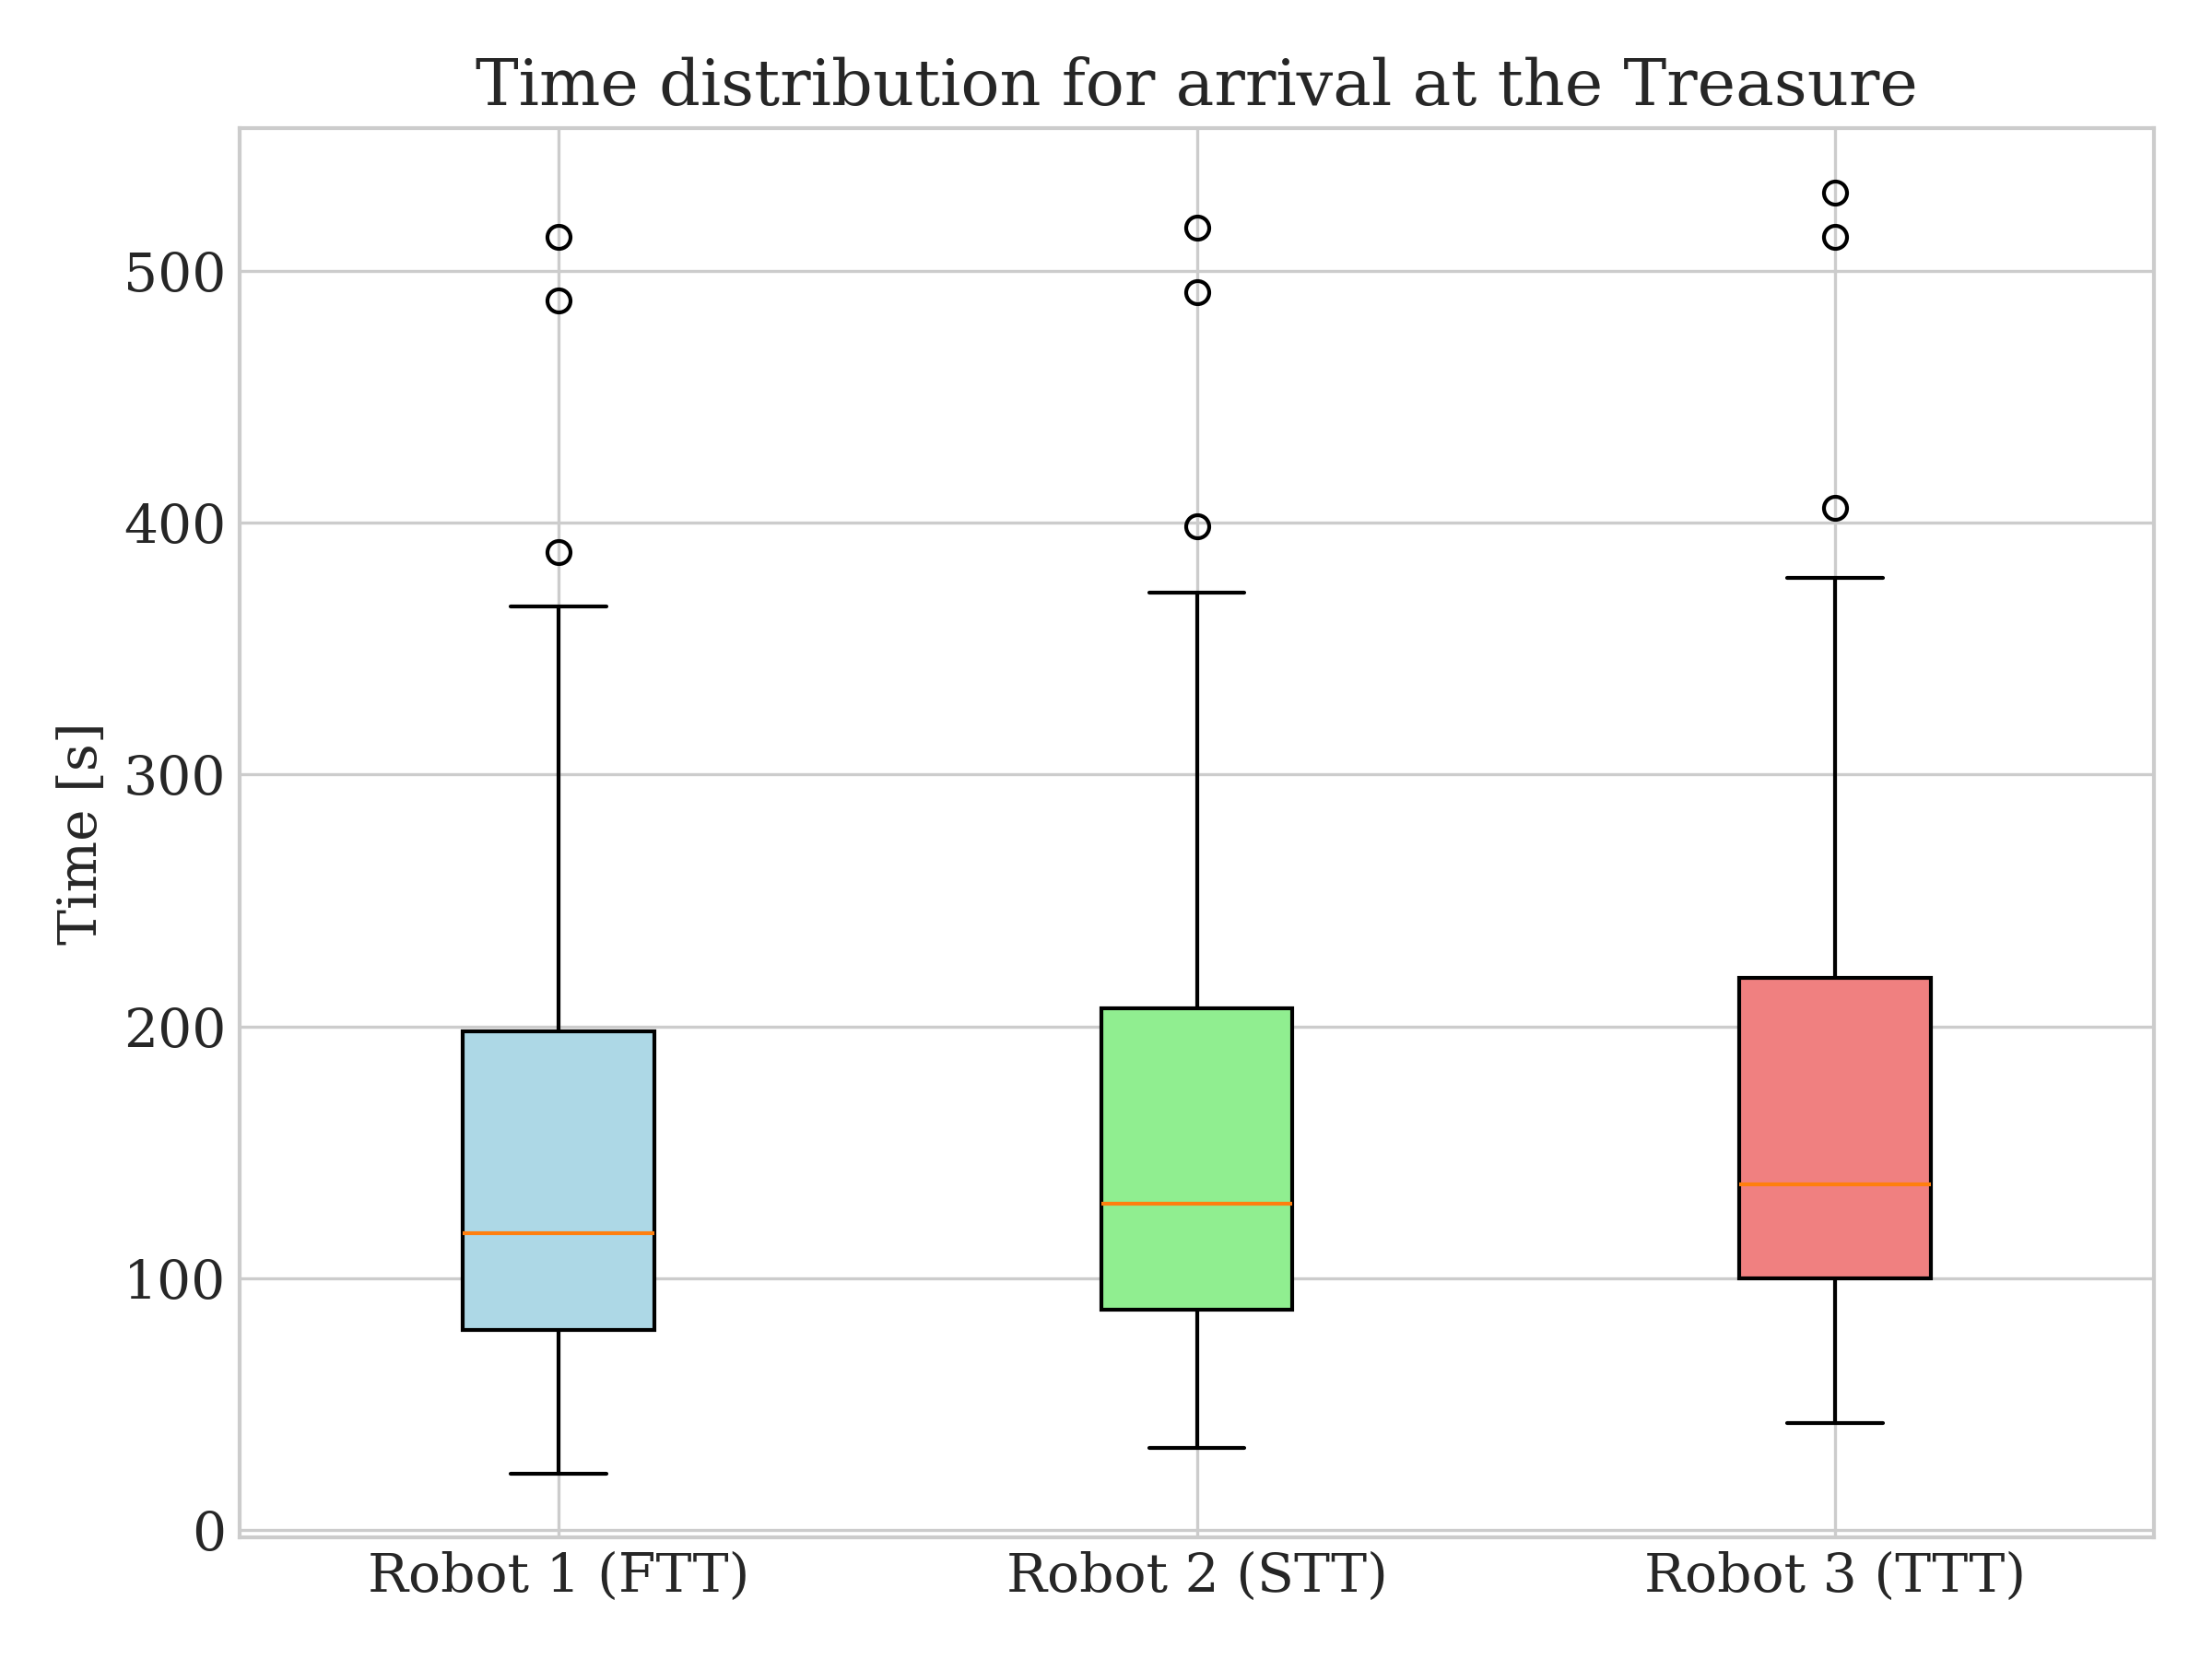
\includegraphics[width=0.8\linewidth]{Figures/grafico_arrivi.png}
    \caption{Time of arrival}
    \label{fig:grafico_arrivi}
\end{figure}

Figure \ref{fig:grafico_arrivi} presents the boxplot distribution of these arrival times. The FTT distribution highlights the efficiency of the Lévy flight combined with the Voronoi partitioning, demonstrating that the environment is explored rapidly without the agents clustering redundantly in the same areas.

More importantly, the STT and TTT distributions validate the robustness of the FSM and the communication network. Once the "Treasure Found" signal is broadcasted, the remaining agents successfully abandon their exploration routines and navigate toward the target. The relatively tight interquartile ranges of the STT and TTT compared to the FTT indicate that robots reliably circumvent static obstacles using the integrated repulsive control, allowing the entire swarm to form the desired ring configuration consistently. 

Another interesting metric to observe is the first discovery distribution among robots. If the robots were to explore randomly, given similar spawning positions, one could expect to find an equal distribution among agents, although simulations report:

\begin{figure}[H]
    \centering
    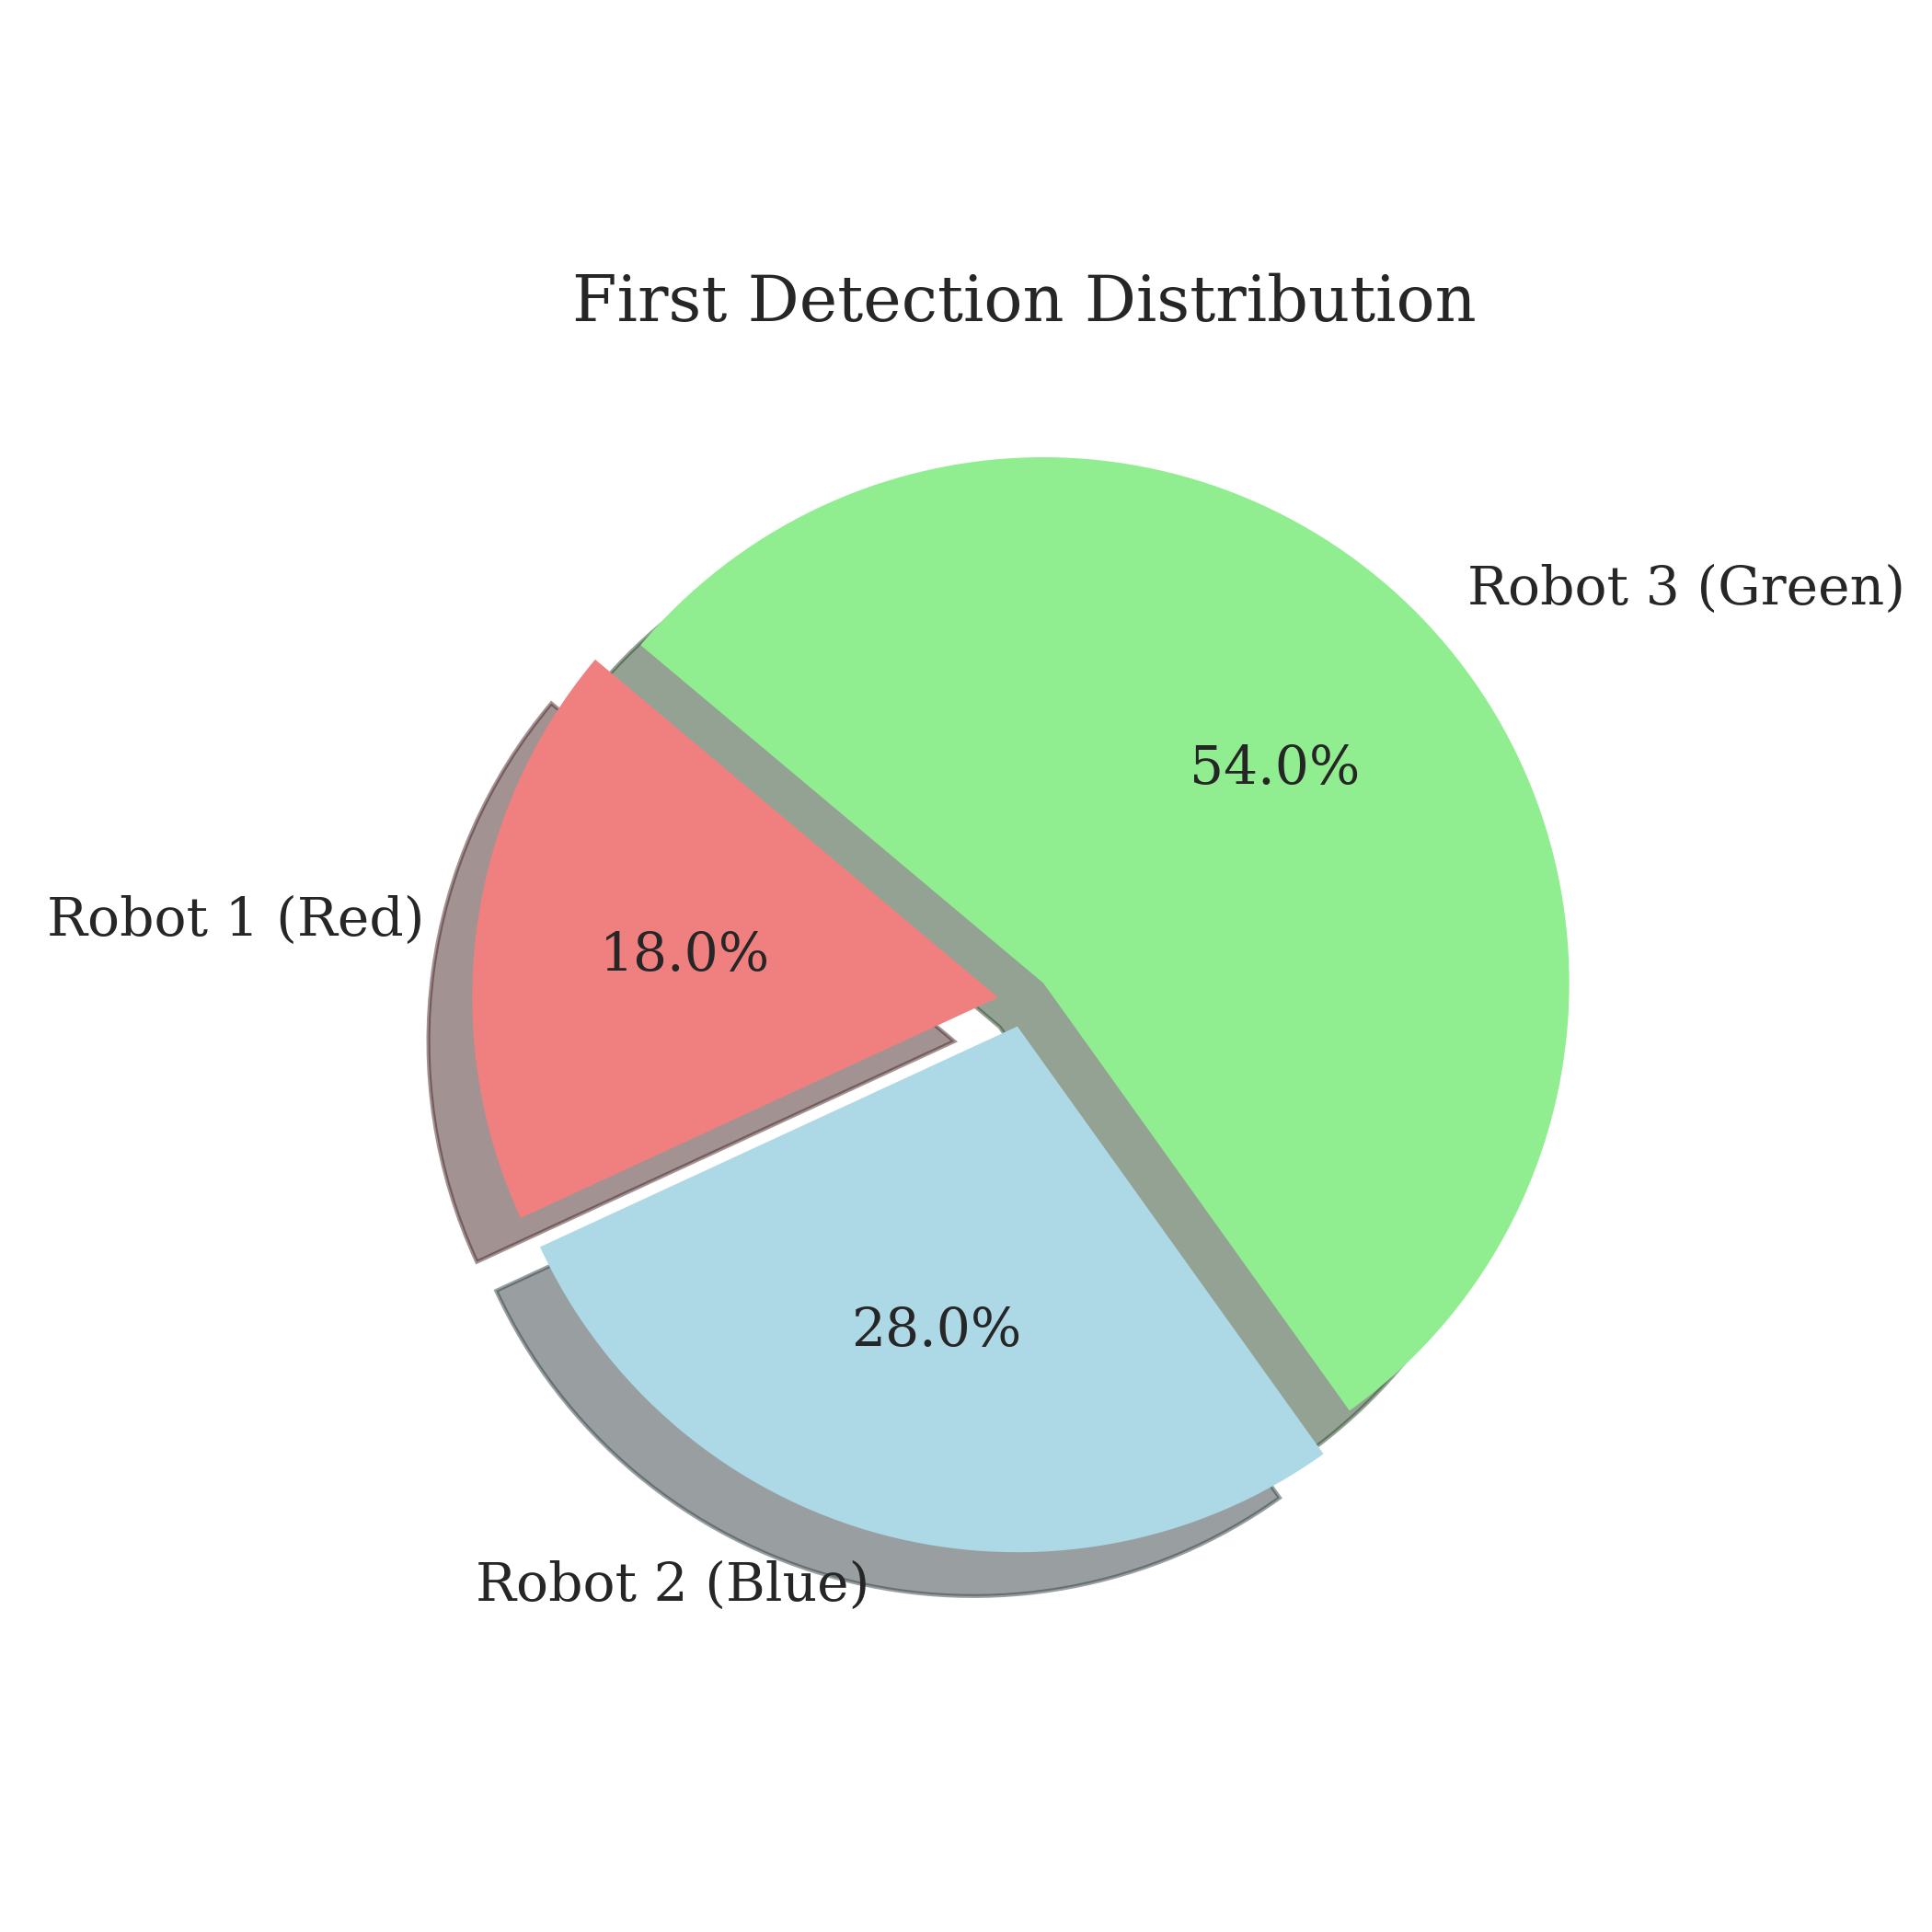
\includegraphics[width=0.8\linewidth]{Figures/grafico_scoperte.png}
    \caption{Treasure discovery distribution}
    \label{fig:distribScoperte}
\end{figure}

Taking into account both Figures \ref{fig:grafico_traiettorie} and \ref{fig:distribScoperte}, it can be possible to motivate why the first detection distribution is not normal. As can be seen by the coverage of the simulated trajectories, the right-hand side of the map is primarily covered by green lines, indicating that the casuality of the Lévy Flight control in this particular environment leads to Robot 3 (green) exploring that particular portion of the map. Robots 1 and 2 tend to wonder around the left-hand side. 


\subsection*{4) Formation convergence}

Now we want to evaluate the circular formation quality by plotting the error between the actual physical distance of each robot from the target and the desired ring radius. Specifically, the distance error for the $i$-th robot at time $t$ is defined as:
\begin{equation}
    e_i(t) = \left| \|\mathbf{p}_i(t) - \mathbf{p}_{\text{target}}\| - r_{\text{ring}} \right|
\end{equation}
where $\mathbf{p}_i(t)$ is the true position of the robot, $\mathbf{p}_{\text{target}}$ is the position of the localized package, and $r_{\text{ring}}$ is the target radius of the circular formation.

\begin{figure}[htbp]
    \centering
    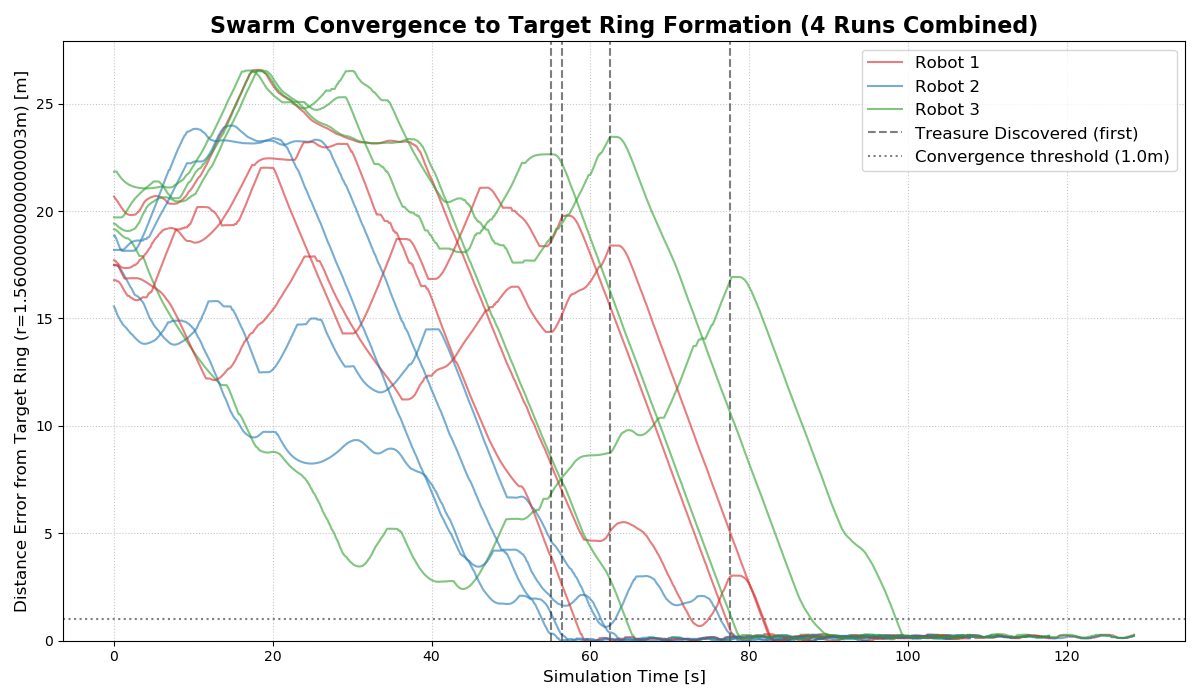
\includegraphics[width=0.75\linewidth]{Figures/Mult_runs_converg_ring.png}
    \caption{Distance error from the target ring radius during exploration and formation phases across multiple independent runs.}
    \label{fig:err_formation}
\end{figure}

As can be seen in Fig. \ref{fig:err_formation}, the simulation data aggregated over multiple independent runs demonstrates the robustness and repeatability of the algorithm. During the initial exploration phase (before the vertical dashed line), the distance error fluctuates randomly as the robots perform their search (e.g., via Lévy flight) to locate the target. 

Once a robot senses the target, the event is broadcasted, and the consensus algorithm rapidly synchronizes the swarm's knowledge. At this precise instant (marked by the dashed line), the Lloyd-based formation control is triggered. The plot clearly shows that, regardless of the robots' arbitrary initial positions across the different runs, the error curves for all agents asymptotically collapse near zero, not perfectly at zero due to uncertainties introduced by the EKF and the LiDAR noise. This proves that the swarm successfully and reliably converges to the desired geometric configuration around the package, within the limits of the system's estimation accuracy.

\subsection*{5) EKF estimation quality}

To evaluate the quality of the Extended Kalman Filter (EKF) estimation, we computed the error between the robot's true state and its estimated state, as shown in Fig. \ref{fig:EKF_err}. 

\begin{figure}[htbp]
    \centering
    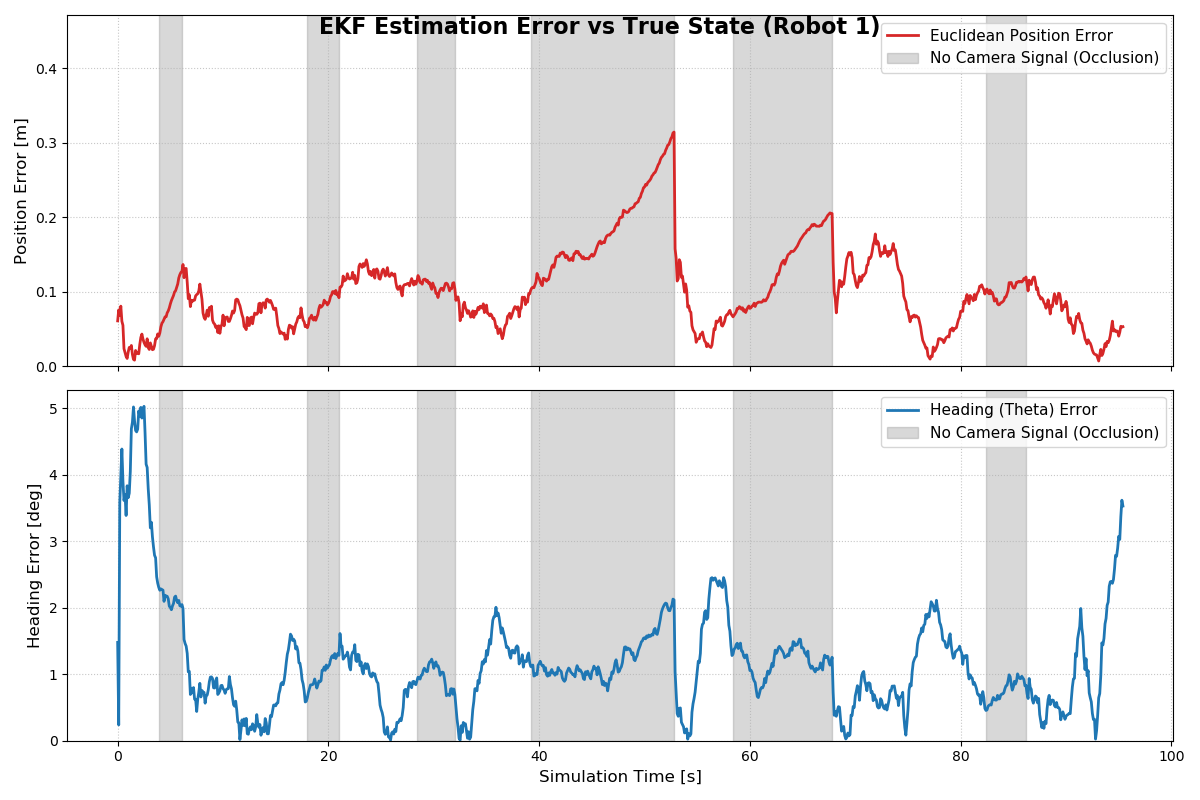
\includegraphics[width=0.75\linewidth]{Figures/EKF_err.png}
    \caption{EKF position and heading tracking error. Shaded areas indicate periods of camera occlusion where the robot relies solely on dead reckoning.}
    \label{fig:EKF_err}
\end{figure}

Specifically, the position error ,as the Euclidean distance between the true and estimated coordinates, and the heading error, as the absolute angular difference, were used.

As highlighted by the shaded regions in the plot, when the robot is occluded by obstacles and loses the global camera signal, the EKF is unable to perform the measurement update step. During these periods, the filter relies entirely on the prediction model (dead reckoning). Consequently, the estimation error inevitably grows due to the continuous accumulation of process noise and odometric drift.

This highlights the critical role of LiDAR-based Voronoi partitioning: it provides reactive obstacle avoidance, preventing collisions even when the global position belief is severely degraded. Moreover, the overall EKF performance remains highly satisfactory, successfully and instantly correcting the accumulated drift as soon as the camera line-of-sight is restored.




\section*{Conclusions}
This project presented a fully decentralized, multi-layered control framework for a swarm of autonomous mobile robots tasked with exploring an unknown environment and localizing a target.

The integration of the Extended Kalman Filter (EKF) proved highly effective in maintaining accurate state estimation by fusing noisy velocity commands with intermittent global camera measurements, ensuring robustness even during periods of visual occlusion. The exploration phase, governed by the Lévy flight strategy and bounded by Voronoi-based spatial partitioning, allowed the agents to efficiently cover the environment while inherently preventing inter-robot collisions.

The transition from exploration to formation control, managed by a robust Finite State Machine, demonstrated the flexibility of the swarm. Upon target detection, the modified Lloyd's algorithm successfully guided the robots into a stable ring formation around the objective, integrating repulsive vectors to navigate safely around static obstacles during the approach.

Finally, the statistical validation conducted through simulations highlighted the strength of the proposed two-tier consensus algorithm. The temporal filtering combined with the Broadcast Gossip network allowed the swarm to dramatically reduce the estimation error over time. The results demonstrated that the collective intelligence of the swarm not only reduces the Time-To-First-Detection (TTFD) variance compared to a single agent, but also achieves an asymptotic convergence of the localization error to near-zero values, proving the overall reliability and scalability of the proposed approach.


\subsection*{Possible Improvements}
Future works on the project would see improvements on both simulation setup and architecture. As a manner of fact, the current framework with Lévy Flight controller can be quite slow in larger or open environments, tracked regions are frequently revisited, bad placed obstacles could lead to the robots getting trapped in a map sector. To overcome this, the implementation of a more sophisticated exploration strategy, such as what is proposed in \cite{zhou2021fuel}, could be considered. This method implements a frontier information structure (FIS) with a hierarchical planner, which allows each individual robot for efficient global coverage. 

Another topic that could be further explored is the communication network. In the current implementation, the Broadcast Gossip algorithm assumes a perfect communication channel with no losses or delays. Future work could investigate the impact of realistic communication constraints, such as packet loss, latency, and limited bandwidth, on the convergence properties of the consensus algorithm. Additionally, exploring alternative consensus strategies that are more robust to communication failures could enhance the reliability of the swarm in real-world scenarios.

%\begin{acknowledgements}
%\blindtext
%\end{acknowledgements}

\section*{Bibliography}
\bibliography{zHenriquesLab-Mendeley}

%% You can use these special %TC: tags to ignore certain parts of the text.
%TC:ignore
%the command above ignores this section for word count
\onecolumn
\newpage

% \section*{Word Counts}
% This section is \textit{not} included in the word count. 
% \subsection*{Notes on Nature Methods Brief Communication}
% \begin{itemize}
% \item Abstract: 3 sentences, 70 words.
% \item Main text: 3 pages, 2 figures, 1000-1500 words, more figures possible if under 3 pages
% \end{itemize}

% \subsection*{Statistics on word count}
% \detailtexcount
% \newpage

%%%%%%%%%%%%%%%%%%%%%%%%%%%%%
% Supplementary Information %
%%%%%%%%%%%%%%%%%%%%%%%%%%%%%
%\captionsetup*{format=largeformat}
%\section{Something about something} \label{note:Note1} 
%\Blindtext

%TC:endignore
%the command above ignores this section for word count

\end{document}
